\chapter{Розповсюдження випромінювання плаского диску в нелінійному середовищі}
\label{ch:nonlinear}

%%%%%%%%%%%%%%%%%%%%%%%%%%%%%%%%%%%%%%%%%%%%%%%%%%%%%%%%%%%%%%%%%%%%%%%%%%%%%%%%
\section{Матеріальні рівняння, як модель нелінійного середовища}

Взаємодію поля крізь середовище з самим собою, завдяки теорії суперпозиції, 
можна представити у вигляді додаткового стороннього джерела поля, що буде 
просторово розподілене в усій області розповсюдження породжувальної 
сильної хвилі. Для сильних хвиль, що мають імпульсну природу 
крім просторового розподілу доводиться розглядати, ще і причинний 
зв'язок. Назвемо таке джерело вторинним, а поле у лінійному наближені 
породжувальною хвилею.

Розглянемо модель, де характер взаємодії електромагнітного поля і середовища 
задається в матеріальних рівняннях, а поляризація та намагніченість 
розглядаються, як джерела електромагнітної індукції.

\begin{equation*}
\vect{D} = \epsilon_0 \vect{E} + \vect{P} \left( \vect{E}, \vect{H} \right) =
\epsilon_0 \vect{E} + \epsilon_0 \chi_e \left( \vect{E}, \vect{H} \right)
\end{equation*}

\begin{equation*}
\vect{B} = \mu_0 \vect{H} + \mu_0 \vect{M} \left( \vect{E}, \vect{H} \right) =
\mu_0 \vect{H} + \mu_0 \chi_m \left( \vect{E}, \vect{H} \right)
\end{equation*}

Так як діелектричні середовища проявляють на порядок слабші магнітні
нелінійні властивості, виключимо нелінійну намагніченість з моделі задля
спрощення \textcolor{red}{[ПОСИЛАННЯ]}.

Виключимо з розглядання гіротропні і не-хіральні середовища, тоді взаємний 
вплив магнітної та електричної індукції зникне і вектор поляризації стане 
функцією лише електричної напруженості, а намагніченість - лише магнітної
напруженості. Також, клас середовищ, що розглядається, обмежимо сталими, 
однорідними та ізотропними властивостями. Тоді, користуючись розкладом за 
малим параметром можна записати вектор поляризації у вигляді нескінченного 
поліному:

\begin{equation} \label{eq:d_voltera}
\vect{D} = \epsilon_0 \vect{E} + \epsilon_0 \chi_e \left( \vect{E} \right) = 
\epsilon_0 \vect{E} + \epsilon_0 \sum_{k=1}^{\infty} \int_0^t
\chi_e^{(k)} (\tau) \vect{E}^k (\tau) d \tau,
\end{equation}
%
де $\chi_e^{(k)} (t) $ коефіцієнти розкладу Вольтера нелінійної функції 
$ \chi_e $ по параметру $ \vect{E} $.

Розклад Вольтера ілюструє затримку у відгуках середовища на помірно сильні 
збудження. Розклад \eqref{eq:d_voltera} може застосовуватись у випадках,
коли породжуюче поле розповсюджуватись у середовищі не змінює його квантовий
стан \textcolor{red}{[ПОСИЛАННЯ]}. Такий тип нелінійності називається 
параметричним та відповідає випадку слабкої нелінійності. Тепер припустимо, 
що нелінійні ефекти в середовищі, що розглядається, не є інерційними за часом 
та породжують індукційний відгук миттєво. Тоді, від розкладу в ряд Вольтера 
перейдемо до Тейлорівського ряду, як моделі нелінійності:

\begin{equation} \label{eq:d_teilor}
\vect{D} = \epsilon_0 \vect{E} + 
\epsilon_0 \sum_{k=1}^{\infty} \chi_e^{(k)} \vect{E}^k (t).
\end{equation}

Застосовуючи властивість симетрії вектору поляризації 
%
\begin{equation}
\vect{P} \left( \vect{E} \right) = - \vect{P} \left( - \vect{E} \right)
\end{equation}
%
помічаємо, що лише непарні доданки ряду Тейлора \eqref{eq:d_teilor} можуть 
бути не нульовими. Тепер, відокремлюючи перший, лінійний, доданок з 
поліному отримаємо наступний вид вектору електричної індукції:

\begin{equation} \label{eq:d_teilor_odd}
\vect{D} = \epsilon_0 \epsilon \vect{E} + 
\epsilon_0 \sum_{k=1}^{\infty} \chi_e^{(2k+1)} \vect{E}^{2k+1} (t).
\end{equation}

Для широкого класу прикладних задач \textcolor{red}{[UPSALA]} розглядається
лише перший нелінійний доданок розкладу. Таким чином отримаємо кубічну 
нелінійну складову вектору поляризації, що зустрічається в оптиці під 
назвою нелінійна поляризація Керра:

\begin{equation} \label{eq:d_kerr}
\vect{D} = 
\epsilon_0 \epsilon \vect{E} + \epsilon_0 \chi_e^{(3)} \vect{E}^{3} = 
\epsilon_0 \epsilon \vect{E} + \vect{P}^\prime.
\end{equation}

Хоча, розклад в ряд Тейлора \eqref{eq:d_teilor_odd} не гарантує зменшення 
впливу кожного наступного доданку, тобто $ \chi_e^{(i)} < \chi_e^{(i+1)} $
на практиці врахування лише першого нелінійного доданку найчастіше дає
гарну точність до наближення слабкої нелінійності і врахуванням доданків
вищих порядків нехтують.

\textcolor{red}{TODO: Які нелінійні ефекти спостерігаються в 
керрівському середовищі?}

Перша складова вектору електричної індукції \eqref{eq:d_kerr} відповідає 
полю при лінійному наближенні $ \vect{E} $, що породжене деяким 
струмом $ \vect{J} $, а другий доданок відповідає нелінійному Керрівському 
відгуку середовища, який згідно з принципом суперпозиції, можна розглянути, 
як деяке поле $ \vect{E}^\prime $, породжене додатковим розподілом струму 
зміщення $ \vect{J}^\prime $ (далі вторинне джерело). Тоді, відповідно до
аналогії зі струмом зміщення, індукований нелінійний вторинний струм

\begin{equation} \label{eq:j_kerr}
\vect{J^\prime} = \partder{\vect{P}^\prime}{t} = 
\epsilon_0 \chi_e^{(3)} \partder{\vect{E}^3}{t}.
\end{equation}

Згідно описаної моделі, деяке стороннє джерело $ \vect{J} $ породжує 
імпульсне електромагнітне поле $ \vect{E} $ та $ \vect{H} $ розраховане
з припущенням лінійності електромагнітної індукції. Це лінійне поле, 
розповсюджуючись зі втратами крізь середовище, формує струм зміщення 
$ \vect{J}^\prime $, який в свою чергу є джерелом поля $ \vect{E}^\prime $ 
та $ \vect{H}^\prime $. Тоді, нелінійна самодія хвилі крізь середовище, 
згідно принципу суперпозиції $ \vect{E} + \vect{E}^\prime $ та 
$ \vect{H} + \vect{H}^\prime $.

Відокремивши лінійну складову з нелінійного доданку вектору індукції 
отримаємо діелектричну проникність поля, що характеризує нелінійні 
властивості середовища $ \chi_e^{(3)} \vect{E}^2 $, що залежить від 
напруженості поля.

Вторинне джерело $ \vect{J}^\prime $ забирає енергію породжуючої хвилі та 
формується частиною енергії втрат $ \vect{E} $, що характеризують середовище.

\textcolor{red}{TODO: Розглянута модель, не пояснює нелінійні ефекти в вакуумі}

Вторинне джерело поля не є реальним джерелом, в прямому розумінні. 
Джерело $ \vect{J^\prime} $ наближено моделює нелінійну природу фізичних 
явищ розповсюдження сильних електромагнітних хвиль. Обмеження, що було 
введено при побудові моделі дозволять розглядати лише саку комбінацію 
середовища і породжувальної хвилі для яких взаємодія відбувається лише
через \textcolor{red}{вид взаємодії коли поле повертає молекули? 
вид взаємодії що іде перед квантовим за енергетичною класифікацією}

Розглянемо в якості породжувальної хвилі $ \vect{E} $ поле, породжене 
пласким диском електричного струму з часовою залежністю у вигляді 
функції Хевісайда - моментальний стрибок амплітуди струму від нуля до 
значення $ A_0 $. 

В контексті цього розділу дане джерело не можна розглядати, як повноцінну 
модель LIRA. Однією з умов роботи лінзових імпульсних антен є те, що матеріал 
лінзи повинен мати більшу діелектричну проникність ніж вільний простір в який 
відбувається випромінювання, а отже нелінійні ефекти проявляться при 
розв'язанні внутрішньої задачі антени більше ніж для зовнішньої. Задачу,
можна вважати моделлю випромінювання модифікованої LIRA, з урахуванням 
нелінійних ефектів про проектуванні та узгоджені антени таким чином, що
її принцип роботи, а тобто вирівнювання сферичного фронту до плаского і 
синфазне збудження розкриву буде виконуватись.

\textcolor{blue}{ \begin{equation*} 
\vect{J^\prime} = 
\vect{\rho_0}    \partder{}{t} P_\rho^\prime    \left( \vect{E} \right) + 
\vect{\varphi_0} \partder{}{t} P_\varphi^\prime \left( \vect{E} \right) + 
\vect{z_0}       \partder{}{t} P_z^\prime       \left( \vect{E} \right) 
\end{equation*} }
%
\textcolor{blue}{ \begin{equation*}
\vect{P^\prime} \left( \vect{E} \right) = \epsilon_0 \chi_e^{(3)} 
\dotprod{ \vect{E} }{ \vect{E} } \cdot \vect{E} 
\end{equation*} }
%
\textcolor{blue}{ \begin{equation*} \begin{aligned}
\vect{P^\prime} \left( \vect{E} \right) = 
\frac{ {A_0}^3 \epsilon_0 \chi_e^{(3)} }{ 8 } \left( \frac{\mu_0 \mu}
{\epsilon_0 \epsilon} \right)^{3/2} \left( {I_1}^2 \cos^2 \varphi + 
\left( I_2 - I_1 \right)^2 \sin^2 \varphi \right) \cdot \\ 
\cdot \Big( \vect{\rho_0} I_1 \cos \varphi - 
\vect{ \varphi_0 } \left( I_2 - I_1 \right) \sin \varphi \Big)
\end{aligned} \end{equation*} }
%
\textcolor{blue}{ \begin{equation*} \begin{aligned}
\vect{P^\prime} \left( \vect{E} \right) = 
\frac{ {A_0}^3 \epsilon_0 \chi_e^{(3)} }{ 8 } \left( \frac{\mu_0 \mu}
{\epsilon_0 \epsilon} \right)^{3/2} \left( {I_1}^2 \cos^2 \varphi + 
\left( I_2 - I_1 \right)^2 \sin^2 \varphi \right) \cdot \\ 
\cdot \Big( \vect{\rho_0} I_1 \cos \varphi - 
\vect{ \varphi_0 } \left( I_2 - I_1 \right) \sin \varphi \Big)
\end{aligned} \end{equation*} }
%
\textcolor{blue}{ \begin{equation*}
\vect{E} = \frac{A_0}{2} \sqrt{\frac{\mu_0 \mu}{\epsilon_0 \epsilon}}
\Big( \vect{\rho_0} I_1 \cos \varphi - 
\vect{ \varphi_0 } \left( I_2 - I_1 \right) \sin \varphi \Big)
\end{equation*} }
%
\textcolor{blue}{ \begin{equation*} \begin{aligned}
\vect{E}^2 = \frac{A_0^2}{4} \frac{\mu_0 \mu}{\epsilon_0 \epsilon}
\Big( I_1^2 \cos^2 \varphi + \left( I_2 - I_1 \right)^2 \sin^2 \varphi \Big)
\end{aligned} \end{equation*} }
%
\textcolor{blue}{ \begin{equation*} \begin{aligned}
\partder{ \vect{E}^2 }{t} = \frac{A_0^2}{4} 
\frac{\mu_0 \mu}{\epsilon_0 \epsilon}
\left( 2 I_1 \partder{I_1}{t} \cos^2 \varphi + 
2 ( I_2 - I_1 ) \left( \partder{I_2}{t} - \partder{I_1}{t} \right) 
\sin^2 \varphi \right)
\end{aligned} \end{equation*} }

Користуючись виразом для вторинного струму Керра \eqref{eq:j_kerr} та 
напруженістю електричного поля \eqref{eq:linear_e_cyl}, запишемо компоненти 
струму.

\textcolor{blue} { \begin{equation*} \begin{aligned}
\partder{P_\rho^\prime}{t}   = \frac{ {A_0}^3 \epsilon_0 \chi_e^{(3)} }{ 8 } 
\left( \frac{\mu_0 \mu} {\epsilon_0 \epsilon} \right)^{3/2} \left(
\left( {I_1}^2 \cos^2 \varphi + ( I_2 - I_1 )^2 \sin^2 \varphi \right)
\partder{I_1}{t} \cos \varphi + \right. \\
\left. + I_1 \cos \varphi \left( 2 I_1 \partder{I_1}{t} \cos^2 \varphi + 
2 ( I_2 - I_1 ) \left( \partder{I_2}{t} - \partder{I_1}{t} \right) 
\sin^2 \varphi \right) \right) = \\ 
= \frac{ {A_0}^3 \epsilon_0 \chi_e^{(3)} }{ 8 } 
\left( \frac{\mu_0 \mu} {\epsilon_0 \epsilon} \right)^{3/2} \left(
\partder{I_1}{t} {I_1}^2 \cos^3 \varphi + \partder{I_1}{t} ( I_2 - I_1 )^2 
\cos \varphi \sin^2 \varphi + \right. \\
\left. + 2 {I_1}^2 \partder{I_1}{t} \cos^3 \varphi + 
2 I_1 ( I_2 - I_1 ) \left( \partder{I_2}{t} - \partder{I_1}{t} \right) 
\cos \varphi \sin^2 \varphi \right)
\end{aligned} \end{equation*} }
%
\begin{equation*} \begin{aligned}
\partder{P_\rho^\prime}{t} = \frac{ {A_0}^3 \epsilon_0 \chi_e^{(3)} }{ 8 } 
\left( \frac{\mu_0 \mu} {\epsilon_0 \epsilon} \right)^{3/2} \left(
3 {I_1}^2 \partder{I_1}{t} \cos^3 \varphi + \right. \\
+ \left. ( I_2 - I_1 ) \cos \varphi \sin^2 \varphi \left( 
\partder{I_1}{t} ( I_2 - I_1 ) + 2 I_1 \left( \partder{I_2}{t} - 
\partder{I_1}{t} \right) \right) \right)
\end{aligned} \end{equation*}
%
\textcolor{blue} { \begin{equation*} \begin{aligned}
\partder{P_\varphi^\prime}{t}   = 
- \frac{ {A_0}^3 \epsilon_0 \chi_e^{(3)} }{ 8 } 
\left( \frac{\mu_0 \mu} {\epsilon_0 \epsilon} \right)^{3/2} \left(
\left( {I_1}^2 \cos^2 \varphi + ( I_2 - I_1 )^2 \sin^2 \varphi \right)
\left( \partder{I_2}{t} - \partder{I_1}{t} \right) \sin \varphi + \right. \\
\left. + (I_2 - I_1) \sin \varphi \left( 2 I_1 \partder{I_1}{t} \cos^2 \varphi + 
2 ( I_2 - I_1 ) \left( \partder{I_2}{t} - \partder{I_1}{t} \right) 
\sin^2 \varphi \right) \right) = \\ 
= - \frac{ {A_0}^3 \epsilon_0 \chi_e^{(3)} }{ 8 } 
\left( \frac{\mu_0 \mu} {\epsilon_0 \epsilon} \right)^{3/2} \left(
{I_1}^2 \left( \partder{I_2}{t} - \partder{I_1}{t} \right) 
\sin \varphi \cos^2 \varphi + \right. \\ \left. 
+ ( I_2 - I_1 )^2 \left( \partder{I_2}{t} - \partder{I_1}{t} \right) 
\sin^3 \varphi + 2 I_1 \partder{I_1}{t} (I_2 - I_1) 
\sin \varphi \cos^2 \varphi + \right. \\ 
+ \left. 2 ( I_2 - I_1 )^2 \left( \partder{I_2}{t} - \partder{I_1}{t} \right) 
\sin^3 \varphi \right)
\end{aligned} \end{equation*} }
%
\begin{equation*} \begin{aligned}
\partder{P_\varphi^\prime}{t} = 
- \frac{ {A_0}^3 \epsilon_0 \chi_e^{(3)} }{ 8 } 
\left( \frac{\mu_0 \mu} {\epsilon_0 \epsilon} \right)^{3/2} \left(
3 ( I_2 - I_1 )^2 \left( \partder{I_2}{t} - \partder{I_1}{t} \right)
\sin^3 \varphi \right. + \\
+ \left. I_1 \sin \varphi \cos^2 \varphi \left( 
I_1 \left( \partder{I_2}{t} - \partder{I_1}{t} \right) + 
2 \partder{I_1}{t} (I_2 - I_1) \right) \right)
\end{aligned} \end{equation*}

Так як поздовжня напруженість електричного поля відсутня 

\begin{equation*} \begin{aligned}
\partder{P_z^\prime}{t} = 0.
\end{aligned} \end{equation*}

Вирази для поперечних компонентів поля стають шматочно-визначеними,
через свої залежності від $ I_1 $ та $ I_2 $, а також від їх похідних в 
кожному з доданків, згрупованих по залежностях від азимутального кута.
Область визначення інтегралів $ I_1 $ та $ I_2 $ відома та має вигляд 
$ S_1 \cup S_2 \cup S_3 $, де кожна з під-областей 
\eqref{eq:s1zone}-\eqref{eq:s3zone} залежить від часу.
Тоді, строго виписана похідна міститиме дельта-функції в точках дотику
часово-просторових областей випромінювання $ S_1 $, $ S_2 $, $ S_3 $.
Користуючись неоднозначністю векторного потенціалу 
\cite[ст. 77]{imp:LandauII} звільнимося від дельта-функцій в виразі для 
похідних від $ I_1 $ та $ I_2 $, тоді

\begin{equation*} \begin{aligned}
\frac{1}{v} \partder{I_\alpha}{t} = 
\frac{1}{v} \partder{ I_\alpha \{ S_{2} \} }{t} 
\Big( H \left( vt^2 - z^2 - (\rho - R)^2 \right)  - 
H \left( vt^2 - z^2 - (\rho + R)^2 \right) \Big),
\end{aligned} \end{equation*}
%
де $ v = c/\sqrt{\epsilon \mu} $ - швидкість світла в середовищі при 
лінійному наближенні вектору поляризації. Таким чином область часу-простору,
де розподілений вторинний струм обмежена лише $ S_2 $, а у всіх точках 
спостереження, що відповідають співвідношенню

\begin{equation*} \begin{aligned}
S^\prime \in S_2 \subset (\rho-R)^2 < vt^2 - z^2 < (\rho+R)^2.
\end{aligned} \end{equation*}

Тоді явні вирази для похідних будуть:

\textcolor{blue}{ \begin{equation*} \begin{aligned}
I_1 \left\{ S_2 \right\} = \frac{\rho^2 + R^2}{4 \pi \rho^2} \arccos 
\frac{c^2 t^2 - z^2 - \rho^2 - R^2}{2 \rho R}  -
\frac{\sqrt{4 \rho^2 R^2 - (\rho^2 + R^2 - c^2t^2 + z^2)^2}}{4 \pi \rho^2} - \\
- \frac{ |\rho^2 - R^2| }{2 \pi \rho^2} 
\arctan \sqrt{ \frac{(\rho - R)^2}{(\rho + R)^2} \cdot
\frac{\left( \rho + R \right)^2 - \left( c^2t^2 - z^2 \right)} 
{\left( c^2t^2 - z^2 \right) - \left( \rho - R \right)^2} }
\end{aligned} \end{equation*} }
%
\textcolor{blue}{ \begin{equation*} \begin{aligned}
\partder{I_1 \left\{ S_2 \right\}}{t} = \frac{\rho^2 + R^2}{4 \pi \rho^2}
\partder{}{t} \arccos \frac{c^2 t^2 - z^2 - \rho^2 - R^2}{2 \rho R} - \\
- \partder{}{t} \frac{\sqrt{4 \rho^2 R^2 - (\rho^2 + R^2 - c^2t^2 + z^2)^2}}
{4 \pi \rho^2} - \\ - \frac{ |\rho^2 - R^2| }{2 \pi \rho^2} \partder{}{t} 
\arctan \sqrt{ \frac{(\rho - R)^2}{(\rho + R)^2} \cdot
\frac{\left( \rho + R \right)^2 - \left( c^2t^2 - z^2 \right)} 
{\left( c^2t^2 - z^2 \right) - \left( \rho - R \right)^2} }
\end{aligned} \end{equation*} }
%
\textcolor{blue}{ \begin{equation*} \begin{aligned}
\partder{}{t} \arccos \frac{c^2 t^2 - z^2 - \rho^2 - R^2}{2 \rho R} = 
- \frac{2 c^2 t}
{ \sqrt{4 \rho^2 R^2 - \left(c^2 t^2 - z^2 - \rho^2 - R^2 \right)^2} }
\end{aligned} \end{equation*} }
%
\textcolor{blue}{ \begin{equation*} \begin{aligned}
- \partder{}{t} \left( \rho^2 + R^2 - c^2t^2 + z^2 \right)^2 = 
- 2 (\rho^2 + R^2 -c^2t^2 + z^2) (-2 c^2 t)
\end{aligned} \end{equation*} }
%
\textcolor{blue}{ \begin{equation*} \begin{aligned}
\partder{}{t} \frac{\sqrt{4 \rho^2 R^2 - (\rho^2 + R^2 - c^2t^2 + z^2)^2}}
{4 \pi \rho^2} = \frac{1}{8 \pi \rho^2} 
\frac{ 4 c^2 t (\rho^2 + R^2 - c^2 t^2 + z^2) }
{ \sqrt{4 \rho^2 R^2 - (\rho^2 + R^2 - c^2t^2 + z^2)^2} } = \\
= \frac{c^2 t}{2 \pi \rho^2} \frac{\rho^2 + R^2 - c^2 t^2 + z^2}
{ \sqrt{4 \rho^2 R^2 - (\rho^2 + R^2 - c^2t^2 + z^2)^2} }
\end{aligned} \end{equation*} }
%
\textcolor{blue}{ \begin{equation*} \begin{aligned}
\partder{}{t} \arctan \sqrt{ \frac{x}{y} } = 
\frac{1}{1 + \frac{x}{y}} \frac{1}{2} 
\sqrt \frac{y}{x} \partder{}{t} \frac{x}{y}
\end{aligned} \end{equation*} }
%
\textcolor{blue}{ \begin{equation*} \begin{aligned}
- \frac{1}{(\rho + R)^2} + \frac{1}{(\rho - R)^2} = 
\frac{- (\rho-R)^2 + (\rho+R)^2 }{ (\rho^2 - R^2)^2 }
\end{aligned} \end{equation*} }
%
\textcolor{blue}{ \begin{equation*} \begin{aligned}
\partder{}{t} \arctan \sqrt{ \frac{(\rho - R)^2}{(\rho + R)^2}
\frac{\left( \rho + R \right)^2 - \left( c^2t^2 - z^2 \right)} 
{\left( c^2t^2 - z^2 \right) - \left( \rho - R \right)^2} } = 
\partder{}{t} \arctan \sqrt{ \frac
{1 - \frac{c^2t^2 - z^2}{\left( \rho + R \right)^2} } 
{ \frac{c^2t^2 - z^2}{ \left( \rho - R \right)^2 } - 1} } = \\
= \frac{1}{1 + \frac{1 - \frac{c^2t^2 - z^2}{\left( \rho + R \right)^2} } 
{ \frac{c^2t^2 - z^2}{ \left( \rho - R \right)^2 } - 1} } \frac{1}{2}
\sqrt{ \frac{ \frac{c^2t^2 - z^2}{ \left( \rho - R \right)^2 } - 1 }
{1 - \frac{c^2t^2 - z^2}{\left( \rho + R \right)^2} } } 
\frac{ - \frac{2 c^2 t}{\left( \rho + R \right)^2} 
\left( \frac{c^2t^2 - z^2}{ \left( \rho - R \right)^2} - 1 \right) - 
\frac{ 2 c^2 t }{ \left( \rho - R \right)^2 } 
\left( 1 - \frac{c^2t^2 - z^2}{\left( \rho + R \right)^2} \right) }
{\left( \frac{c^2t^2 - z^2}{ \left( \rho - R \right)^2 } - 1 \right)^2} = \\
= - c^2 t \frac{ \frac{c^2t^2-z^2}{(\rho-R)^2} - 1 }
{ \frac{c^2t^2-z^2}{(\rho-R)^2} - 1 + 1 - 
\frac{c^2t^2 - z^2}{\left( \rho + R \right)^2} }
\sqrt{ \frac{ \frac{c^2t^2 - z^2}{ \left( \rho - R \right)^2 } - 1}
{1 - \frac{c^2t^2 - z^2}{\left( \rho + R \right)^2} } } \frac
{ \frac{c^2t^2 - z^2}{ \left( \rho^2 - R^2 \right)^2 } - \frac{1}{(\rho+R)^2} + 
\frac{1}{(\rho-R)^2} - \frac{ c^2t^2 - z^2 }{ \left( \rho^2 - R^2 \right)^2 } }
{ \left( \frac{c^2t^2 - z^2}{ \left( \rho - R \right)^2} - 1 \right)^2 } = \\
= - \frac{4 \rho R c^2 t}{ \left( \rho^2 - R^2 \right)^2 } 
\frac{ 1 }{ \frac{c^2t^2-z^2}{(\rho-R)^2} - 
\frac{c^2t^2 - z^2}{\left( \rho + R \right)^2} }
\sqrt{ \frac{ \frac{c^2t^2 - z^2}{ \left( \rho - R \right)^2 } - 1}
{1 - \frac{c^2t^2 - z^2}{\left( \rho + R \right)^2} } } \frac
{ 1 }{ \frac{c^2t^2 - z^2}{ \left( \rho - R \right)^2} - 1 } = \\
= - \frac{c^2 t}{ c^2 t^2 - z^2 } \frac{1} { 
\sqrt{ 1 - \frac{c^2t^2 - z^2}{(\rho + R)^2 } } 
\sqrt{ \frac{c^2t^2 - z^2}{ (\rho - R)^2 } - 1} }
\end{aligned} \end{equation*} }
%
\textcolor{blue}{ \begin{equation*} \begin{aligned}
\partder{ I_1 \{ S_2 \} }{t} = - \frac{c^2 t}{2 \pi \rho^2}
\frac{\rho^2 + R^2}
{ \sqrt{4 \rho^2 R^2 - \left(c^2 t^2 - z^2 - \rho^2 - R^2 \right)^2} } - \\
- \frac{c^2 t}{2 \pi \rho^2} \frac{\rho^2 + R^2 - c^2 t^2 + z^2}
{ \sqrt{4 \rho^2 R^2 - (\rho^2 + R^2 - c^2t^2 + z^2)^2} } + \\ 
+ \frac{ c^2 t }{2 \pi \rho^2} \frac{|\rho^2 - R^2|}{ c^2 t^2 - z^2 } \frac{1} 
{ \sqrt{ 1 - \frac{c^2t^2 - z^2}{(\rho + R)^2 } } 
\sqrt{ \frac{c^2t^2 - z^2}{ (\rho - R)^2 } - 1} }
\end{aligned} \end{equation*} }
%
\begin{equation} \begin{aligned} \label{eq:i1_partder}
\frac{1}{v} \partder{ I_1 \{ S_2 \} }{t} = \frac{ vt }{2 \pi \rho^2} 
\frac{ (\rho^2 - R^2)^2  (v^2 t^2 - z^2)^{-1} } 
{ \sqrt{ (\rho + R)^2 - v^2t^2 + z^2 } 
\sqrt{ v^2t^2 - z^2 - (\rho - R)^2 } } - \\
- \frac{vt}{2 \pi \rho^2} \frac{2 (\rho^2 + R^2) - (v^2 t^2 - z^2)}
{ \sqrt{4 \rho^2 R^2 - (v^2t^2 - z^2 - \rho^2 - R^2)^2} };
\end{aligned} \end{equation}
%
\textcolor{blue}{ \begin{equation*} \begin{aligned}
\partder{ I_2 \{ S_2 \} }{t} = \frac{1}{\pi} \partder{}{t} \arccos 
\frac{c^2t^2 - z^2 + \rho^2 - R^2}{2 \rho \sqrt{c^2t^2 - z^2}} = \\
= - \frac{1}{\pi} \frac{1} { \sqrt{ 1 - \frac{ (c^2t^2 - z^2 + \rho^2 - R^2)^2 }
{4 \rho^2 (c^2t^2 - z^2)^2} } } \frac{1}{2 \rho} \partder{}{t} 
\frac{c^2t^2 - z^2 + \rho^2 - R^2} {\sqrt{c^2t^2 - z^2}} = \\
= - \frac{1}{2 \rho \pi} \frac{1} 
{ \sqrt{ 1 - \frac{ (c^2t^2 - z^2 + \rho^2 - R^2)^2 }
{4 \rho^2 (c^2t^2 - z^2)} } } \frac{2c^2t \sqrt{c^2t^2 - z^2} - 
\frac{c^2t}{\sqrt{c^2t^2 - z^2}} (c^2t^2 - z^2 + \rho^2 - R^2)
}{c^2t^2 - z^2} = \\ = - \frac{c^2 t}{2 \pi \rho} \frac{1} 
{ \sqrt{ 1 - \frac{ (c^2t^2 - z^2 + \rho^2 - R^2)^2 }
{4 \rho^2 (c^2t^2 - z^2)} } } \frac{2 \sqrt{c^2t^2 - z^2} - 
\frac{c^2t^2 - z^2 + \rho^2 - R^2}{\sqrt{c^2t^2 - z^2}}}{c^2t^2 - z^2} = \\
= - \frac{c^2 t}{2 \pi \rho (c^2t^2 - z^2)} \frac{ 2 \sqrt{c^2t^2 - z^2} - 
\frac{c^2t^2 - z^2 + \rho^2 - R^2}{\sqrt{c^2t^2 - z^2}} } 
{ \sqrt{ 1 - \frac{ (c^2t^2 - z^2 + \rho^2 - R^2)^2 }
{4 \rho^2 (c^2t^2 - z^2)} } } = \\
= - \frac{c^2 t}{\pi (c^2t^2 - z^2) } 
\frac{ 2 (c^2t^2 - z^2) - (c^2t^2 - z^2 + \rho^2 - R^2) } 
{ \sqrt{ 4 \rho^2 (c^2t^2 - z^2) - (c^2t^2 - z^2 + \rho^2 - R^2)^2 } } = \\
= - \frac{c^2 t}{\pi (c^2t^2 - z^2) } \frac{ c^2t^2 - z^2 -  \rho^2 + R^2 } 
{ \sqrt{ 4 \rho^2 (c^2t^2 - z^2) - (c^2t^2 - z^2 + \rho^2 - R^2)^2 } }
\end{aligned} \end{equation*} }
%
\begin{equation} \begin{aligned} \label{eq:i2_partder}
\frac{1}{v} \partder{ I_2 \{ S_2 \} }{t} = 
- \frac{vt}{\pi (v^2t^2 - z^2) } \frac{ v^2t^2 - z^2 - \rho^2 + R^2 } 
{ \sqrt{ 4 \rho^2 (v^2t^2 - z^2) - (v^2t^2 - z^2 + \rho^2 - R^2)^2 } }.
\end{aligned} \end{equation}

Графічно можемо визначити, що проекція вторинного струм обернена за знаком 
відносно тієї ж проекції компоненти напруженості електричного поля.

\begin{figure}[h] \begin{center}
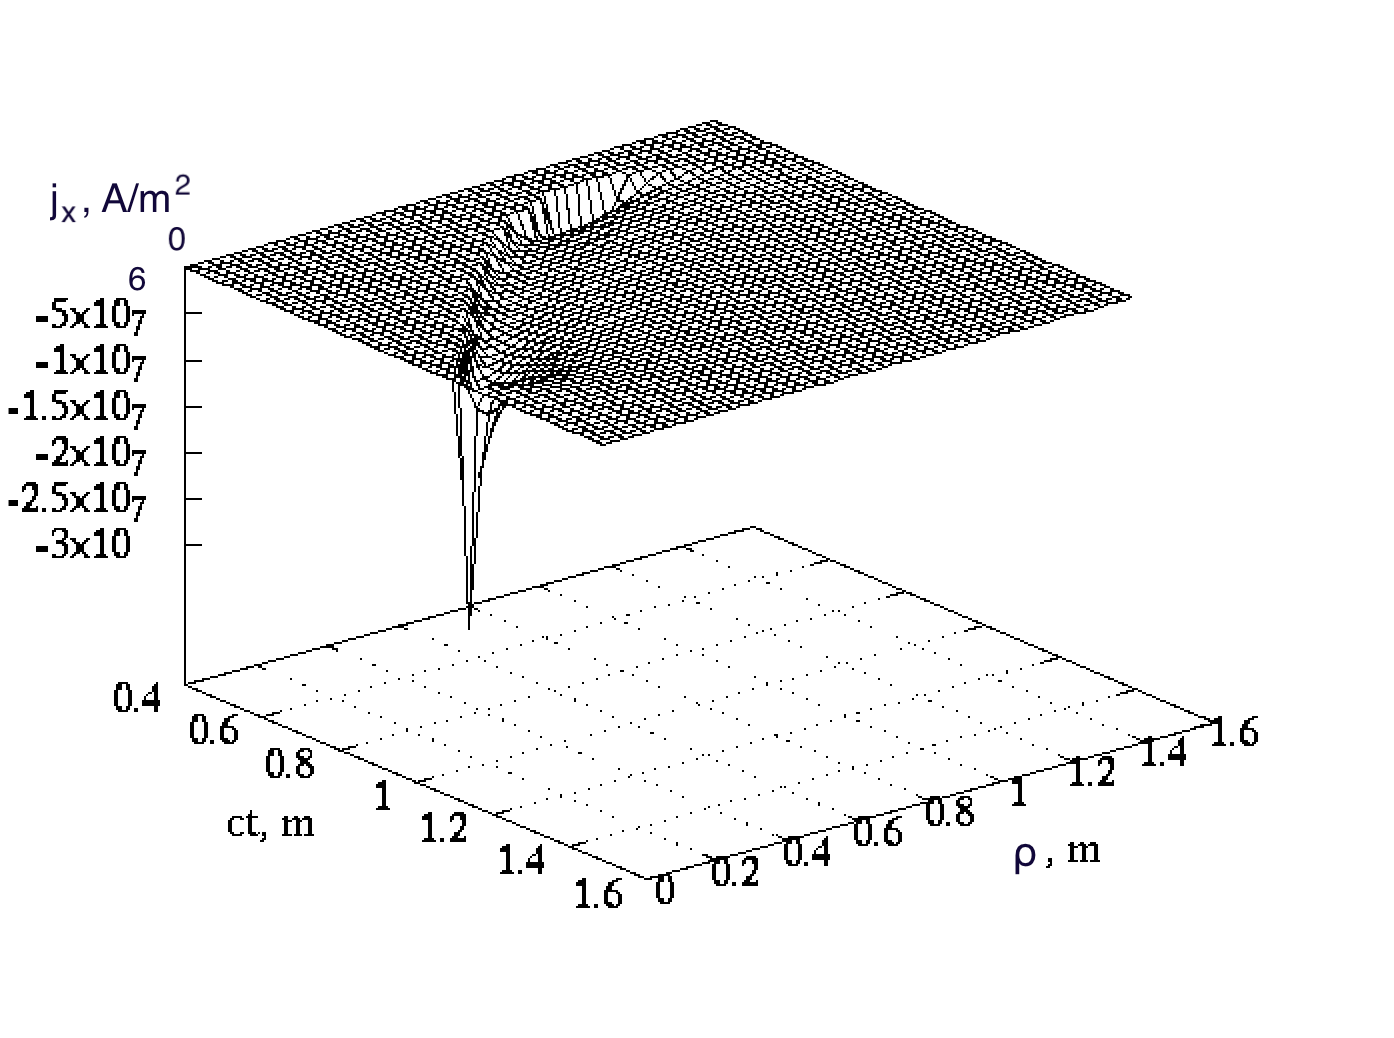
\includegraphics[scale=0.5]{Jperp_A1}
\caption{Нелінійність амплітуди вторинного джерела}
\label{fig:jx_secondary}
\end{center} \end{figure}

З виразів \eqref{eq:i1_partder}, \eqref{eq:i2_partder} очевидна нелінійна 
залежність струму від $ A_0 $.

%%%%%%%%%%%%%%%%%%%%%%%%%%%%%%%%%%%%%%%%%%%%%%%%%%%%%%%%%%%%%%%%%%%%%%%%%%%%%%%%
\section{Енергетичний розподіл поля плаского диску в лінійному наближенні}

Вторинний електричний струм розподілений в усьому напівпросторі $ z > 0 $,
але за рахунок згасання енергії з відстанню в межах $ [1/R, 1/R^2] $ (в 
залежності від напрямку спостереження) можемо обмежити область де треба 
враховувати нелінійні ефекти за рахунок високої концентрації енергії. Для 
визначення параметричних меж застосування введеної моделі нелінійності та 
оцінки границі зони, де нелінійні ефекти треба враховувати, розглянемо 
енергетичні характеристики поля в ближній зоні

Тепер розглянемо енергетичний розподіл від поля плаского диску при різних
часових залежностей $ f(t) $ стороннього струму. Побудова класичної 
енергетичної діаграми спрямованості мало інформативне дослідження нелінійних
ефектів - в даній роботі важливим є енергетичний розподіл в ближній зоні.

Розглянемо густину енергії електромагнітного поля $ \vect{E} $, збудженого 
пласким диском електричного струму з довільною часовою залежністю $ f(t) $ за 
визначенням \cite{imp:Schantz2018}, нехтуючи при цьому енергетичним внеском 
$ \vect{H} $ спираючись на відсутність нелінійного внеску останньої.

\begin{equation} \label{eq:energy}
W = \frac{\epsilon_0}{2} \int_0^\infty \vect{E}^2 dt
\end{equation}

Користуючись властивостями перехідної функції можемо обмежити
область інтегрування за часом, а також спростити підінтегральний вираз

\begin{equation} \label{eq:energy}
W = \frac{\epsilon_0}{2} \frac{\mu_0 \mu}{\epsilon_0 \epsilon}
\int_{ct_1}^{c\tau_0+ct_3} \left( E_\rho^2 + E_\varphi^2 \right) dt
\end{equation}

Також оцінено енергію перехідної функції, а тобто \ref{eq:energy} при 
часовій залежності сигналу у вигляді функції Гевісайда $ f(t) = H(t) $:

\textcolor{blue}{ \begin{equation*} \begin{aligned}
\vect{E}^2 = \frac{A_0^2}{4} \frac{\mu_0 \mu}{\epsilon_0 \epsilon}
\Big( I_1^2 \cos^2 \varphi + \left( I_2 - I_1 \right)^2 \sin^2 \varphi \Big)
\end{aligned} \end{equation*} }
%
\begin{equation} \label{eq:energy_tr}
W_{tr} = \frac{\epsilon_0 A_0^2}{8} \frac{\mu_0 \mu}{\epsilon_0 \epsilon}
\int_{ct_1}^{ct_3}  \Big( I_1^2 \cos^2 \varphi + 
\left( I_2 - I_1 \right)^2 \sin^2 \varphi \Big) dt.
\end{equation}

Розглядаючи особливий випадок \ref{eq:energy_tr} для $ \rho = 0 $, помічаємо,
що енергія випромінювання плаского диску, завжди лежить у наступних межах для 
сигналів з часовою залежністю $ f(t) $ з областю значень 
$ \left[ -1, 1 \right] $ та тривалістю $ \tau_0 $:

\textcolor{blue}{ \begin{equation*}
\left. W \right|^{\rho=0} = \frac{\epsilon_0 A_0^2}{32} 
\frac{\mu_0 \mu}{\epsilon_0 \epsilon} \Big( \sqrt{R^2+z^2} - z \Big)
\end{equation*} }
%
\textcolor{blue}{ \begin{equation*}
\int_{ct_1}^{c\tau_0+ct_3} 
\left( \int_0^t f(\tau) d \tau < \tau_0 \right) dt < \tau_0 R
\end{equation*} }
%
\begin{equation}
0 \leq W_{max} \left( \tau_0, f(t), \vect{r} \right) < 
\frac{\epsilon_0 \tau_0 R A_0^2}{32} \frac{\mu_0 \mu}{\epsilon_0 \epsilon},
\end{equation}
%
де $ W_{max} $ - густина енергії, $ \tau_0 $ - ефективна тривалість імпульсу 
за визначеною метрикою, $ A_0 $ - максимальна амплітуда сигналу, $ R $ - 
радіус апертури, а вираз під коренем - імпеданс у середовищі розповсюдження 
хвилі.

Будуватимемо поперечні зрізи значень енергій для різних довжин імпульсів та 
для різних відстаней від джерела. Для збереження кутового розміру зрізів 
візьмемо його $ z + 2R $.

\textcolor{red}{ TODO: побудувати поздовжні та поперечні енергетичні зрізи
для декількох $ f(t) $ }

\textcolor{red}{ Як видно з рисунків, форма збудження має значний вплив на 
розподіл енергії у ближній зоні, де вклад нелінійної поправки найбільший, а 
отже обмежувати область врахування вторинного струму на основі енергетичних 
характеристик породжувальної хвилі треба з урахуванням часової залежності 
струму }

\textcolor{red}{ TODO: можна строго порівняти діаграму спрямованості 
отриману в часовій області з діаграмою Баума, а також оцінити її відхилення 
в ближній зоні }

\begin{figure}
\subfloat[а]{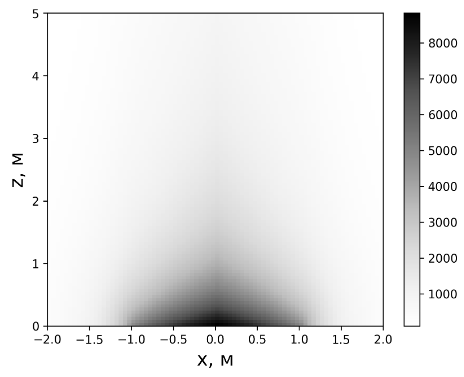
\includegraphics[width = 3in]{Wtr_xz}} 
\subfloat[б]{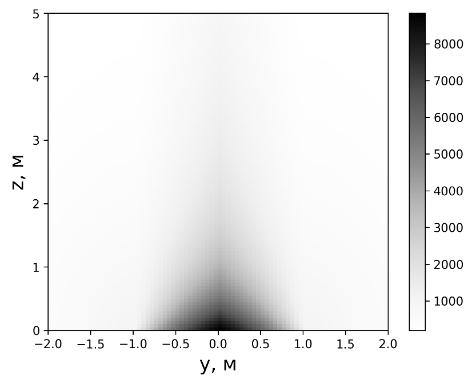
\includegraphics[width = 3in]{Wtr_yz}}
\caption{Розподіл густини енергії}
\label{fig:gauss_shape}
\end{figure}

%%%%%%%%%%%%%%%%%%%%%%%%%%%%%%%%%%%%%%%%%%%%%%%%%%%%%%%%%%%%%%%%%%%%%%%%%%%%%%%%
\section{Модовий розподіл Керрівської поправки}

Застосуємо метод еволюційних рівнянь для розв'язання задачі випромінювання 
вторинним струмом \eqref{eq:j_kerr}. Для цього, спершу, запишемо модовий
розподіл джерела, який є правою частиною рівняння Клейна-Гордона. 

\textcolor{blue} { \begin{equation*}
j_m \left( r, t; \nu \right) = \frac{\sqrt{\mu_0}}{2\pi} 
\int \limits_{0}^{2\pi} d \varphi \int \limits_0^\infty \rho d \rho 
\vect{j_0} \crossprod{ \nabla_\perp \Psi_m^* }{ \vect{z_0} }
\end{equation*} }
%
\textcolor{blue} { \begin{equation*} 
\vect{J^\prime} = 
\vect{\rho_0}    \partder{}{t} P_\rho^\prime    \left( \vect{E} \right) + 
\vect{\varphi_0} \partder{}{t} P_\varphi^\prime \left( \vect{E} \right) + 
\vect{z_0}       \partder{}{t} P_z^\prime       \left( \vect{E} \right) 
\end{equation*} }
%
\textcolor{blue} { \begin{equation*} \begin{aligned}
\crossprod{ \nabla_\perp \Psi_m^* }{ \vect{z_0} } =
- \vect{\rho_0} i m e^{-im\varphi} \frac{J_m (\nu \rho)}{\rho \sqrt{\nu}}
- \vect{\varphi_0} \sqrt{\nu} e^{-im\varphi} 
\frac{J_{m-1} (\nu \rho) - J_{m+1} (\nu \rho)}{2}
\end{aligned} \end{equation*} }
%
\textcolor{blue} { \begin{equation*} \begin{aligned}
\vect{J^\prime} \crossprod{ \nabla_\perp \Psi_m^* }{ \vect{z_0} } = 
- i e^{-im\varphi} m \frac{J_m (\nu \rho)}{\rho \sqrt{\nu}}
\partder{}{t} P_\rho^\prime \left( \vect{E} \right) - \\
- \sqrt{\nu} e^{-im\varphi} \frac{J_{m-1} (\nu \rho) - J_{m+1} (\nu \rho)}{2}
\partder{}{t} P_\varphi^\prime \right)
\end{aligned} \end{equation*} }

\begin{equation*} \begin{aligned}
j_m = - \frac{\sqrt{\mu_0}}{2\pi} 
\int_{0}^{2\pi} d \varphi \int \limits_{0}^{\infty} \rho d \rho
e^{-im\varphi} \left( i  m \frac{J_m (\nu \rho)}{\rho \sqrt{\nu}}
\partder{j_\rho^\prime}{t} + \sqrt{\nu}
\frac{J_{m-1} (\nu \rho) - J_{m+1} (\nu \rho)}{2}
\partder{j_\varphi^\prime}{t} \right)
\end{aligned} \end{equation*}

Спершу, перейдемо від комплексної області визначення модового розподілу 
до уявної. Згрупувавши доданки за тригонометричними функціями,
знайдемо інтеграли за азимутальним кутом $ \varphi $, користуючись 
аналітичними інтегралами \eqref{eq:int_exp3}, \eqref{eq:int_exp4}, 
\eqref{eq:int_exp5}, \eqref{eq:int_exp6}. Отримаємо вирази для інтегралів
від компонентів вектору вторинного нелінійного струму з ядром інтегралу у 
вигляді комплексної експоненти.

\textcolor{blue} { \begin{equation*} \begin{aligned}
\int_0^{2\pi} e^{-i m \varphi} \cos^3 \varphi d \varphi = 
\frac{\pi}{4} \delta_{m,-3} + \frac{\pi}{4} \delta_{m,3} + 
\frac{3 \pi}{4} \delta_{m,-1} + \frac{3 \pi}{4} \delta_{m,1}
\end{aligned} \end{equation*} }
%
\textcolor{blue} { \begin{equation*} \begin{aligned}
\int_0^{2\pi} e^{-i m \varphi} \cos \varphi \sin^2 \varphi d \varphi = 
\frac{\pi \delta_{m,1} }{4} + \frac{\pi \delta_{m,-1} }{4} - 
\frac{\pi \delta_{m,-3} }{4} - \frac{\pi \delta_{m,3} }{4}
\end{aligned} \end{equation*} }
%
\textcolor{blue} { \begin{equation*} \begin{aligned}
\int_{0}^{2 \pi} d \varphi e^{-im \varphi} \partder{P_\rho^\prime}{t} = 
\frac{ {A_0}^3 \epsilon_0 \chi_e^{(3)} }{ 8 } \int_{0}^{2\pi} d \varphi
e^{-im\varphi} \left( \frac{\mu_0 \mu} {\epsilon_0 \epsilon} \right)^{3/2} 
\left( 3 {I_1}^2 \partder{I_1}{t} \cos^3 \varphi + \right. \\
+ \left. ( I_2 - I_1 ) \cos \varphi \sin^2 \varphi \left( 
\partder{I_1}{t} ( I_2 - I_1 ) + 2 I_1 \left( \partder{I_2}{t} - 
\partder{I_1}{t} \right) \right) \right) = \\
= \frac{ {A_0}^3 \epsilon_0 \chi_e^{(3)} }{ 8 } 
\left( \frac{\mu_0 \mu} {\epsilon_0 \epsilon} \right)^{3/2}
\left( \frac{3 \pi}{4} {I_1}^2 \partder{I_1}{t} \left( \delta_{m,-3} + 
\delta_{m,3} + 3 \delta_{m,-1} + 3 \delta_{m,1} \right) + \right. \\
+ \frac{\pi }{4} \left. ( I_2 - I_1 ) \left( \delta_{m,1} + 
\delta_{m,-1} - \delta_{m,-3} - \delta_{m,3} \right) \left( 
\partder{I_1}{t} ( I_2 - I_1 ) + 2 I_1 \left( \partder{I_2}{t} - 
\partder{I_1}{t} \right) \right) \right)
\end{aligned} \end{equation*} }
%
\begin{equation*} \begin{aligned}
\frac{\epsilon_0 \chi_e^{(3)}}{2 \pi} \int_{0}^{2\pi} d \varphi 
e^{-im \varphi} \partder{P_\rho^\prime}{t} = 
\frac{ {A_0}^3 \epsilon_0 \chi_e^{(3)}}{ 64 } 
\left( \frac{\mu_0 \mu} {\epsilon_0 \epsilon} \right)^{3/2} \cdot \\ 
\cdot \left( 3 {I_1}^2 \partder{I_1}{t} \left( \delta_{m,-3} + 
\delta_{m,3} + 3 \delta_{m,-1} + 3 \delta_{m,1} \right) + \right. \\
+ \left. ( I_2 - I_1 ) \left( \delta_{m,1} + \delta_{m,-1} - 
\delta_{m,-3} - \delta_{m,3} \right) \left( 
\partder{I_1}{t} ( I_2 - I_1 ) + 2 I_1 \left( \partder{I_2}{t} - 
\partder{I_1}{t} \right) \right) \right)
\end{aligned} \end{equation*}
%
\textcolor{blue} { \begin{equation*} \begin{aligned}
\int_{0}^{2\pi} e^{-i m \varphi} \sin^3 \varphi d \varphi = 
\frac{3 \pi i}{4} \delta_{m,-1} - \frac{3 \pi i}{4} \delta_{m,1} - 
\frac{\pi i}{4} \delta_{m,-3} + \frac{\pi i}{4} \delta_{m,3}
\end{aligned} \end{equation*} }
%
\textcolor{blue} { \begin{equation*} \begin{aligned}
\int_0^{2\pi} e^{-i m \varphi} \sin \varphi \cos^2 \varphi d \varphi = 
\frac{\pi i }{4} \delta_{m,-1} - \frac{\pi i }{4} \delta_{m,1} -
\frac{\pi i }{4} \delta_{m,3} + \frac{\pi i }{4} \delta_{m,-3}
\end{aligned} \end{equation*} }
%
\textcolor{blue} { \begin{equation*} \begin{aligned}
\int_{0}^{2 \pi} d \varphi e^{-im \varphi} \partder{P_\varphi^\prime}{t} = \\
= - \frac{ {A_0}^3 \epsilon_0 \chi_e^{(3)} }{ 8 } 
\int_{0}^{2 \pi} d \varphi e^{-im \varphi}
\left( \frac{\mu_0 \mu} {\epsilon_0 \epsilon} \right)^{3/2} \left(
3 ( I_2 - I_1 )^2 \left( \partder{I_2}{t} - \partder{I_1}{t} \right)
\sin^3 \varphi \right. + \\
+ \left. I_1 \sin \varphi \cos^2 \varphi \left( 
I_1 \left( \partder{I_2}{t} - \partder{I_1}{t} \right) + 
2 \partder{I_1}{t} (I_2 - I_1) \right) \right) = 
- \frac{ {A_0}^3 \epsilon_0 \chi_e^{(3)} }{ 8 } \cdot \\ 
\cdot \left( \frac{\mu_0 \mu} {\epsilon_0 \epsilon} \right)^{3/2} \left(
\frac{3 \pi i}{4} ( I_2 - I_1 )^2 \left( \partder{I_2}{t} - 
\partder{I_1}{t} \right) \left( 3 \delta_{m,-1} - 3 \delta_{m,1} - 
\delta_{m,-3} + \delta_{m,3} \right) \right. + \\
+ \left. \frac{\pi i}{4} I_1 \left( \delta_{m,-1} - \delta_{m,1} - 
\delta_{m,3} + \delta_{m,-3} \right) \left( 
I_1 \left( \partder{I_2}{t} - \partder{I_1}{t} \right) + 
2 \partder{I_1}{t} (I_2 - I_1) \right) \right)
\end{aligned} \end{equation*} }
%
\begin{equation*} \begin{aligned}
\frac{\epsilon_0 \chi_e^{(3)}}{2 \pi} \int_{0}^{2 \pi} d \varphi 
e^{-im \varphi} \partder{P_\varphi^\prime}{t} = 
- \frac{ {A_0}^3 \epsilon_0 \chi_e^{(3)}  i}{ 64 }
\left( \frac{\mu_0 \mu} {\epsilon_0 \epsilon} \right)^{3/2} \cdot \\ 
\cdot \left( 3 ( I_2 - I_1 )^2 \left( \partder{I_2}{t} - 
\partder{I_1}{t} \right) \left( 3 \delta_{m,-1} - 3 \delta_{m,1} - 
\delta_{m,-3} + \delta_{m,3} \right) \right. + \\
+ \left. I_1 \left( \delta_{m,-1} - \delta_{m,1} - 
\delta_{m,3} + \delta_{m,-3} \right) \left( 
I_1 \left( \partder{I_2}{t} - \partder{I_1}{t} \right) + 
2 \partder{I_1}{t} (I_2 - I_1) \right) \right)
\end{aligned} \end{equation*}

Як видно з останніх виразів, інтригування за кутом $ \varphi $ дає дискретний 
модовий розподіл вторинного струму.  Також помічаємо, що у розподілах присутні 
лише моді з номерами $ \pm 1 $ та $ \pm 3 $ - вклад вторинного струму в інші
моди відсутній. Випишемо окрему кожну з ненульових мод розподілу вторинного 
струму. Для цього введемо нові змінні:

\begin{equation} \begin{aligned} \label{eq:alpha}
\alpha = 3 {I_1}^2 \partder{I_1}{t}
\end{aligned} \end{equation}

\begin{equation} \begin{aligned} \label{eq:beta}
\beta = ( I_2 - I_1 ) \left( \partder{I_1}{t} ( I_2 - I_1 ) + 
2 I_1 \left( \partder{I_2}{t} - \partder{I_1}{t} \right) \right)
\end{aligned} \end{equation}

\begin{equation} \begin{aligned} \label{eq:gamma}
\gamma = 3 ( I_2 - I_1 )^2 \left( \partder{I_2}{t} - \partder{I_1}{t} \right)
\end{aligned} \end{equation}

\begin{equation} \begin{aligned} \label{eq:lambda}
\lambda = I_1^2 \left( \partder{I_2}{t} - 
\partder{I_1}{t} \right) + 2 I_1 \partder{I_1}{t} (I_2 - I_1)
\end{aligned} \end{equation}

Запишемо модовий розподіл струму через нові позначення, спростивши вираз 
можна отримати:

\textcolor{blue} { \begin{equation*} \begin{aligned}
j_m = - \frac{\sqrt{\mu_0}}{2\pi} 
\int_0^{2\pi} d \varphi \int \limits_0^\infty \rho d \rho
e^{-im\varphi} \left( i m \frac{J_m (\nu \rho)}{\rho \sqrt{\nu}}
j_\rho^\prime + \sqrt{\nu}
\frac{J_{m-1} (\nu \rho) - J_{m+1} (\nu \rho)}{2}
j_\varphi^\prime \right)
\end{aligned} \end{equation*} }
%
\textcolor{blue} { \begin{equation*} \begin{aligned}
j_m = - \frac{\sqrt{\mu_0}}{2\pi} 
\int_0^{2\pi} d \varphi \int \limits_0^\infty \rho d \rho 
e^{-im\varphi} \cdot \\ \cdot 
\left( i \sqrt{\nu} \frac{J_{m-1} (\nu \rho) + J_{m+1} (\nu \rho)}{2}
j_\rho^\prime + \sqrt{\nu} 
\frac{J_{m-1} (\nu \rho) - J_{m+1} (\nu \rho)}{2}
j_\varphi^\prime \right)
\end{aligned} \end{equation*} }
%
\textcolor{blue} { \begin{equation*} \begin{aligned}
j_m = - \frac{\sqrt{\mu_0} \sqrt{\nu}}{4\pi} 
\int_0^{2\pi} d \varphi \int \limits_0^\infty \rho d \rho 
e^{-im\varphi} \Big(
J_{m-1} (\nu \rho) ( i j_\rho^\prime + j_\varphi^\prime ) +
J_{m+1} (\nu \rho) ( i j_\rho^\prime - j_\varphi^\prime ) \Big)
\end{aligned} \end{equation*} }
%
\begin{equation} \begin{aligned}
j_1 = \frac{i A_0^3 \sqrt{\mu_0} \epsilon_0 \chi_e^{(3)} \sqrt{\nu}}{128}
\left( \frac{\mu_0 \mu}{\epsilon_0 \epsilon} \right)^{3/2}
\int_0^\infty \rho d \rho \cdot \\ \cdot
\Big( J_0 (\nu \rho) ( 3 \alpha + \beta + 3 \gamma + \lambda) + 
J_2 (\nu \rho) ( 3 \alpha + \beta - 3 \gamma - \lambda ) \Big)
\end{aligned} \end{equation}
%
\textcolor{blue} { \begin{equation*} \begin{aligned}
j_{-1} = \frac{i A_0^3 \sqrt{\mu_0} \epsilon_0 \chi_e^{(3)} \sqrt{\nu}}{128}
\left( \frac{\mu_0 \mu}{\epsilon_0 \epsilon} \right)^{3/2}
\int_0^\infty \rho d \rho \cdot \\ \cdot
\Big( J_2 (\nu \rho) ( 3 \alpha + \beta - 3 \gamma - \lambda ) + 
J_0 (\nu \rho) ( 3 \alpha + \beta + 3 \gamma + \lambda ) \Big)
\end{aligned} \end{equation*} }
%
\begin{equation} \begin{aligned}
j_{-1} = j_{1}
\end{aligned} \end{equation}
%
\textcolor{blue} { \begin{equation*} \begin{aligned}
j_{3} = - \frac{i A_0^3 \sqrt{\mu_0} \epsilon_0 \chi_e^{(3)} \sqrt{\nu}}{128}
\left( \frac{\mu_0 \mu}{\epsilon_0 \epsilon} \right)^{3/2}
\int_0^\infty \rho d \rho \cdot \\ \cdot
\Big( J_2 (\nu \rho) ( \alpha - \beta - \gamma + \lambda) + 
J_4 (\nu \rho) ( \alpha - \beta + \gamma - \lambda) \Big)
\end{aligned} \end{equation*} }
%
\begin{equation*} \begin{aligned}
j_{-3} = - \frac{i A_0^3 \sqrt{\mu_0} \epsilon_0 \chi_e^{(3)} \sqrt{\nu}}{128}
\left( \frac{\mu_0 \mu}{\epsilon_0 \epsilon} \right)^{3/2}
\int_0^\infty \rho d \rho \cdot \\ \cdot
\Big( J_4 (\nu \rho) ( \alpha - \beta + \gamma - \lambda) + 
J_2 (\nu \rho) ( \alpha - \beta - \gamma + \lambda) \Big)
\end{aligned} \end{equation*}
%
\begin{equation} \begin{aligned}
j_{-3} = j_{3}
\end{aligned} \end{equation}

\begin{figure}[htbp] \begin{center}
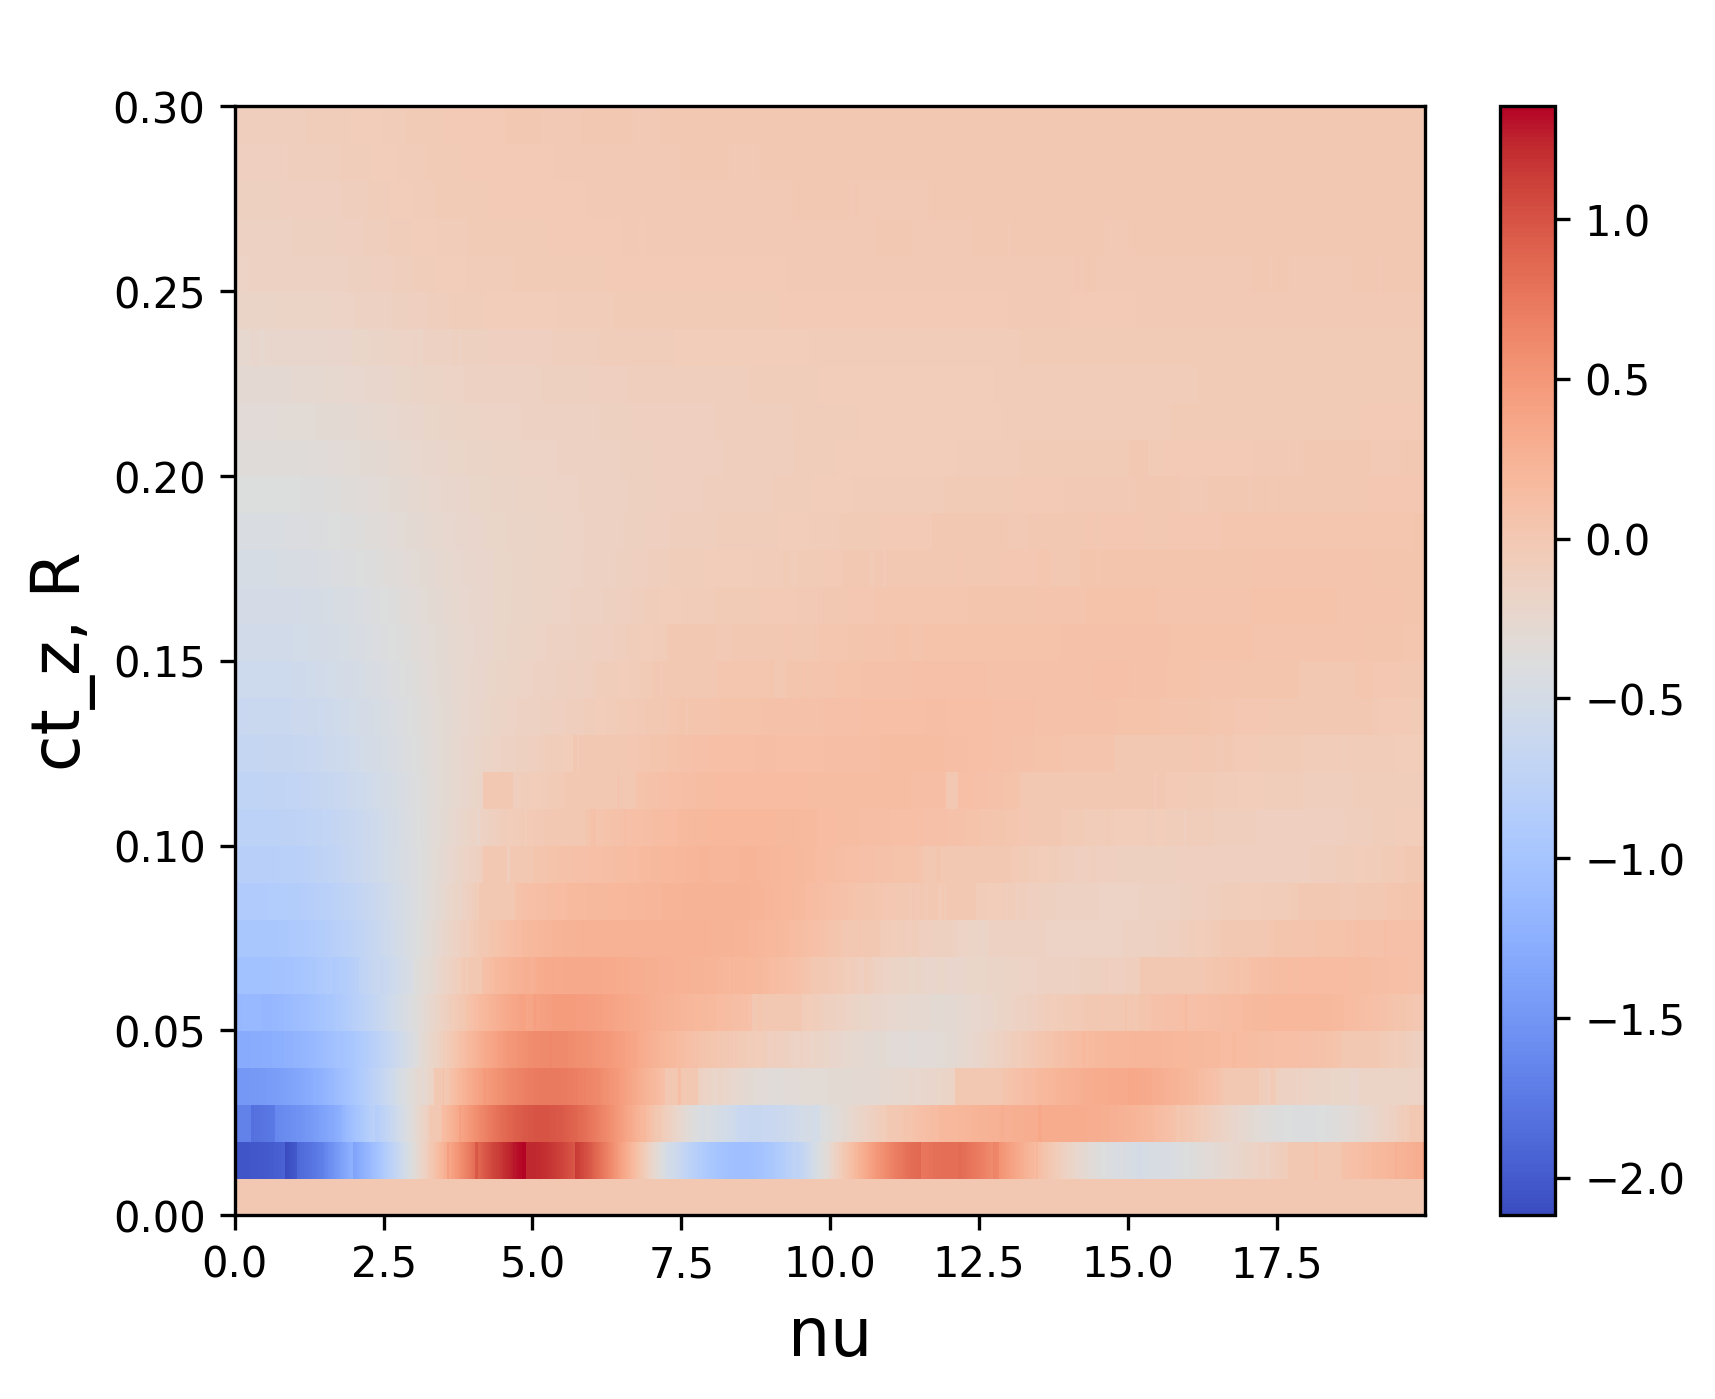
\includegraphics[scale=1.0]{normed_j1}
\caption{Нормована швидкість зміни моди $ j_1 $ у часі} \label{fig:mode1}
\end{center} \end{figure}

\begin{figure}[htbp] \begin{center}
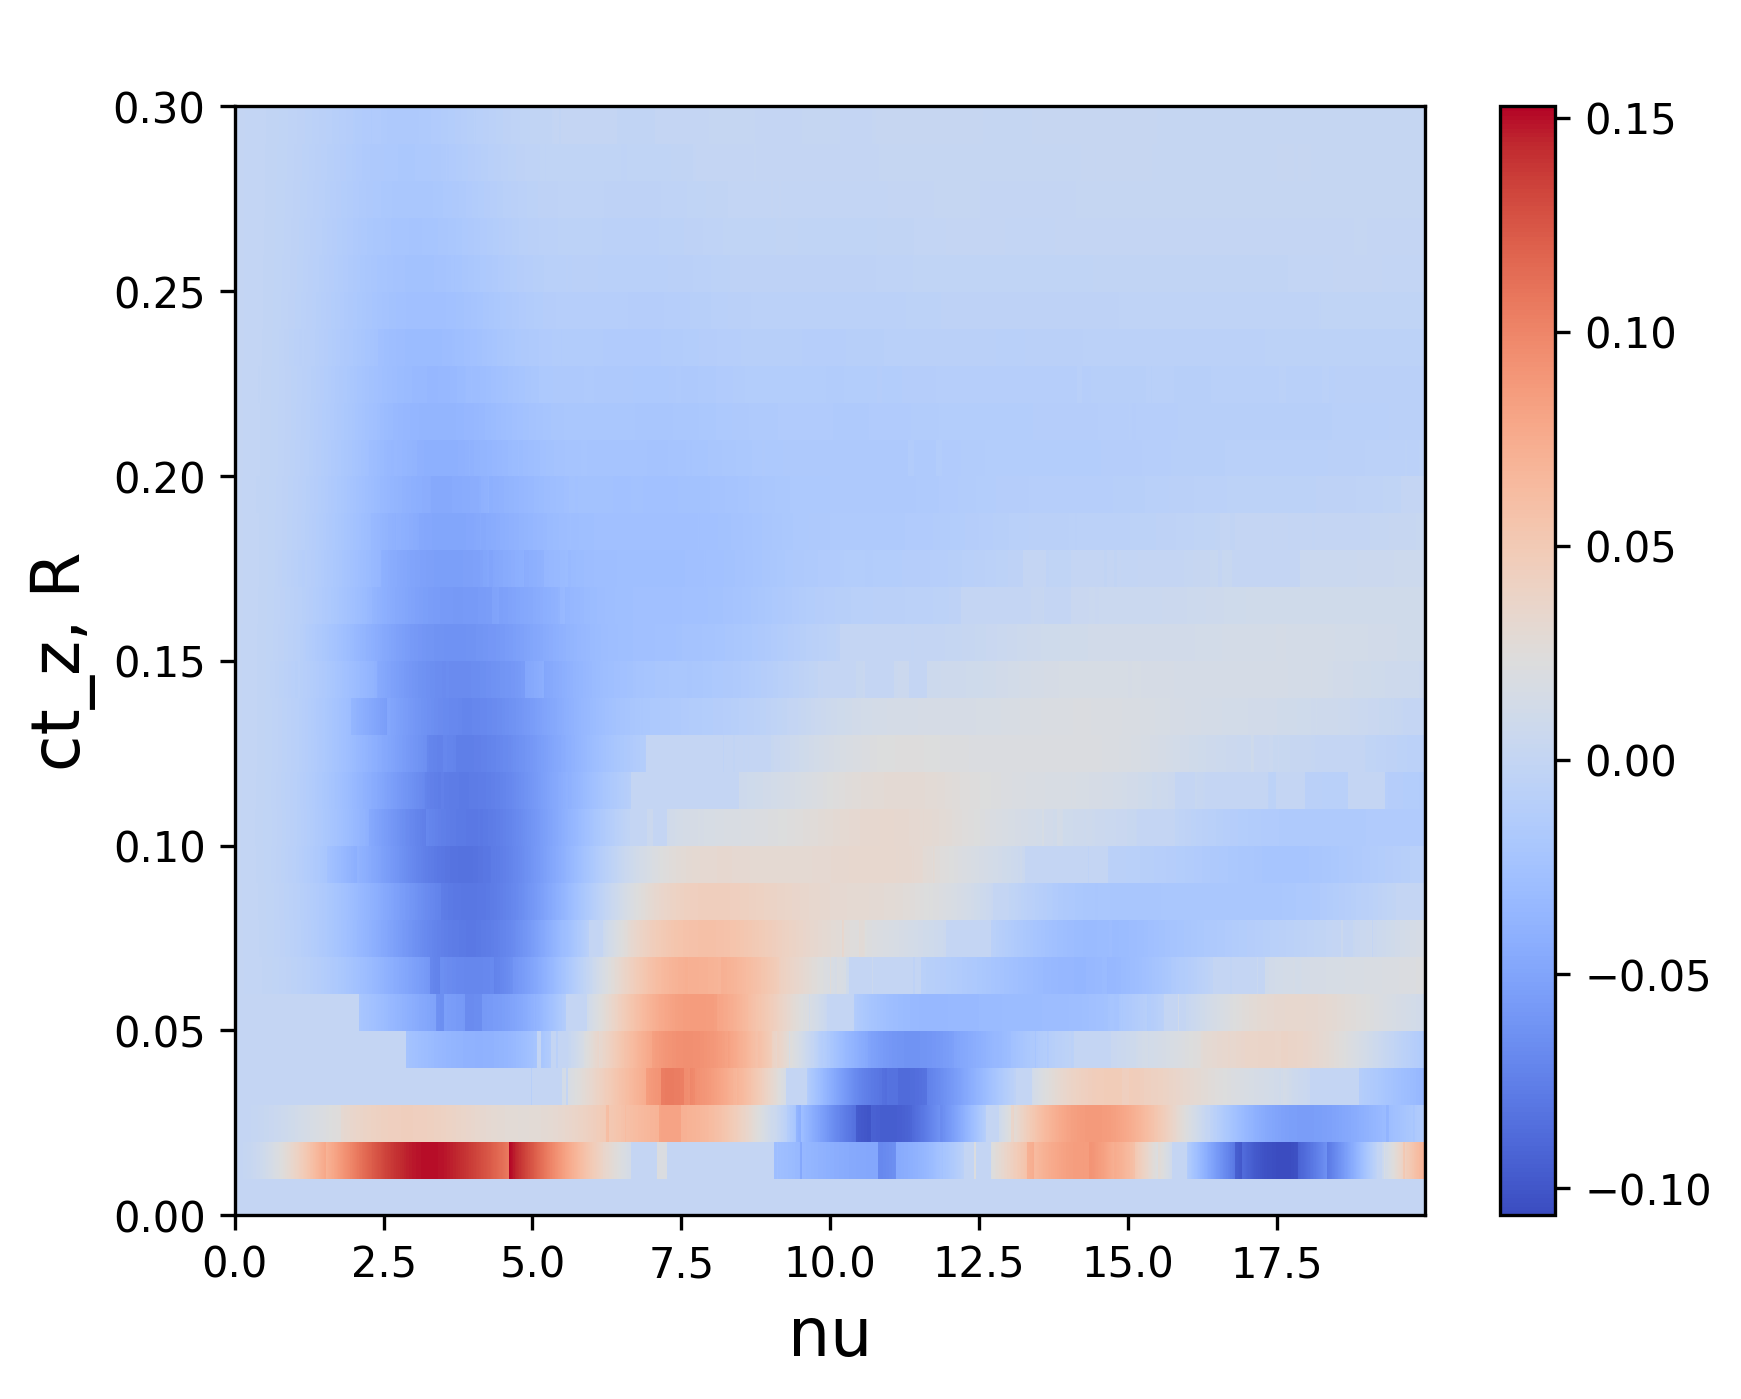
\includegraphics[scale=1.0]{normed_j3}
\caption{Нормована швидкість зміни моди $ j_3 $ у часі} \label{fig:mode3}
\end{center} \end{figure}

На рис.~\ref{fig:mode1} і на рис.~\ref{fig:mode3} зображено величину модового 
струму нормовану на час $ j_m / ct $ для різних значень $ ct-z $ та $ \nu $.
$ j_m / ct $ нормування вибрано задля того, щоб щоб зручно показати модовий 
струм, як функцію всіх його змінних на одному графіку. Якщо розглянути вторинне
електричне поле як суперпозицію двох окремих хвиль (з кутовою модою $ m = 1 $ 
та $ m = 3 $), помічаємо, що внесок хвилі при $ m = 1 $ на порядок більший.

Для чисельного розрахунку невласного інтегралу по $ \rho $, що містяться в 
модових розподілах струму $ j_m $ зручно звузити межі інтегрування 
користуючись областю визначення під-інтегральної функцій $ S_2 $:

\textcolor{blue} { \begin{equation*} \begin{aligned}
(\rho - R)^2 \leq v^2t^2 - z^2 \leq (\rho + R)^2
\end{aligned} \end{equation*} }
%
\textcolor{blue} { \begin{equation*} \begin{aligned}
| \rho - R | - \sqrt{v^2t^2 - z^2} \leq 0 \leq \rho + R - \sqrt{v^2t^2 - z^2}
\end{aligned} \end{equation*} }
%
\textcolor{blue} { \begin{equation*} \begin{aligned}
- R - \sqrt{v^2t^2 - z^2} \leq - \rho \leq R - \sqrt{v^2t^2 - z^2}
\end{aligned} \end{equation*} }
%
\textcolor{blue} { \begin{equation*} \begin{aligned}
R + \sqrt{v^2t^2 - z^2} \geq \rho \geq - R + \sqrt{v^2t^2 - z^2}
\end{aligned} \end{equation*} }
%
\begin{equation} \begin{aligned}
\left| \sqrt{v^2t^2 - z^2} - R \right| \leq \rho \leq \sqrt{v^2t^2 - z^2} + R.
\end{aligned} \end{equation}

Задля відокремлення розмірних коефіцієнтів перевизначимо модовий розподіл 
струму:

\begin{equation} \begin{aligned}
j_m = - \frac{i A_0^3 \sqrt{\mu_0} \epsilon_0 \chi_e^{(3)} \sqrt{\nu}}{128}
\left( \frac{\mu_0 \mu}{\epsilon_0 \epsilon} \right)^{3/2} \hat{j_m}.
\end{aligned} \end{equation}

Так як поздовжня компонента вторинного струму $ J_z $ відсутня, рівняння 
Клейна-Гордона відносно поздовжнього електричного еволюційного коефіцієнту 
є однорідним, що згідно методом функції Рімана дає нульовий розв'язок для
цього коефіцієнту. Отже, як і у лінійному наближенні, електромагнітне поле 
з урахуванням ефектів слабкої нелінійності залишається ТЕ типу:

\textcolor{blue}{ \begin{equation*}
- \partial_{ct}(\mu I_n^e) - \partial_z V_n^e + \chi^2 e_n = 0
\end{equation*} }
%
\textcolor{blue}{ \begin{equation*}
\frac{\epsilon \mu}{ \sqrt{\epsilon_0 \mu_0}} 
\frac{\partial^2 e_n}{\partial t^2} - 
\frac{\partial^2 e_n}{\partial z^2} + \chi^2 e_n = 
- \frac{\sqrt{\mu_0}}{2 \pi c} 
\int_0^{2\pi} d \varphi 
\int_0^\infty \rho d \rho \Phi_n^* (\chi) \partder{J_z}{t} = 0
\end{equation*} }
%
\textcolor{blue}{ \begin{equation*}
e_n (z, t; \chi) = \iint_S j_n (t',z', \chi) G(t,t',z,z') dt' dz' = 0
\end{equation*} }
%
\textcolor{blue}{ \begin{equation*}
I_n^e = - \partial_{ct} (\epsilon e_n) - 
\frac{\sqrt{\mu_0}}{2 \pi} \int_0^{2\pi} d \varphi 
\int_0^{\infty} \rho d \rho \Phi_n^* (\chi) J_z
\end{equation*} }
%
\textcolor{blue}{ \begin{equation*}
\partial_{z} e_n = V_n^e
\end{equation*} }
%
\begin{equation} \label{eq:e_evolution}
e_n (z, t; \nu) = V_n^e (z, t; \nu) = I_n^e (z, t; \nu) = 0
\end{equation}

Пошук виразів для еволюційних коефіцієнтів починаємо з поздовжнього 
магнітного коефіцієнту $ h_m $. Для розглянутої фізичної моделі ізотропного
та стаціонарного середовища без втрат коефіцієнт $ h_m $ є розв'язком 
рівняння Клейна-Гордона. В лінійному випадку це рівняння містить електричну 
і магнітну сприйнятливості; для нелінійної нотації скористаємось поняттям 
ефективної сприйнятливості та методикою запропонованою R. Ziolkowski
\cite{imp:Ziolkowski1993}.

\begin{equation} \label{eq:klein_gordon_nl}
\frac{(\epsilon + \chi_e^{(3)}) \mu}{c^2} 
\frac{\partial^2 h_m}{\partial t^2} - 
\frac{\partial^2 h_m}{\partial z^2} + 
\nu^2 h_m = j_m (t',z'; \nu),
\end{equation}
%
де $ j_m (t',z'; \nu) $ - мода $ m $ дискретного розподілу стороннього 
джерела, $ \chi_e^{(3)} $ - відносна нелінійна електрична сприйнятливість 
середовища третього порядку, а величина $ \epsilon + \chi_e^{(3)} $ в 
літературі зустрічається, як ефективна нелінійна Керрівська сприйнятливість 
\cite{imp:Ziolkowski1993}. Тоді, розв'язком \eqref{eq:klein_gordon_nl} за 
методом функції Рімана буде \eqref{eq:klein_gordon_sol} з ядром у вигляді 
функції Рімана

\begin{equation*}
G(t,t',z,z') = \frac{v}{2} H \left( v (t-t') - (z-z') \right)
J_0 \left( \nu \sqrt{v^2 (t-t')^2 - (z-z')^2} \right),
\end{equation*}
%
де $ v $ - швидкість світла в середовищі з урахуванням нелінійного 
Керрівського сповільнення

\begin{equation}
v = \frac{c}{\sqrt{ \left(\epsilon + \chi_e^{(3)}\right) \mu}} = 
\left( \epsilon_0 
\left( \epsilon + \chi_e^{(3)} \right) \mu_0 \mu \right)^{-1/2}.
\end{equation}

Для отримання нелінійних поправок до напруженості електричного поля достатньо 
поперечного модового коефіцієнту $ V_m^h $, який лінійно залежить від $ h_m $

\textcolor{blue}{ \begin{equation*} 
h_m (z, t; \nu) = \iint_S j_m (t',z') G(t,t',z,z') dt' dz',
\end{equation*} }
%
\textcolor{blue}{ \begin{equation*}
V_m^h = - \mu \partial_{ct} (h_m)
\end{equation*} }
%
\textcolor{blue} { \begin{equation*} \begin{aligned} 
V_m^h = - \mu \partial_{ct} \int_0^\infty \int_0^\infty j_m (t',z') G dz' dt'
\end{aligned} \end{equation*} }
%
\textcolor{blue} { \begin{equation*} \begin{aligned} 
V_m^h = - \frac{v \mu}{2c}
\partder_{t} \int_0^\infty dz' \int_0^\infty 
dt' H \left( v (t-t') - (z-z') \right) \cdot \\
\cdot J_0 \left( \nu \sqrt{v^2 (t-t')^2 - (z-z')^2} \right) j_m (t',z')
\end{aligned} \end{equation*} }
%
\textcolor{blue} { \begin{equation*} \begin{aligned} 
V_m^h = - \frac{1}{2} \sqrt{\frac{\mu}{\epsilon + \chi_e^{(3)}}}
\partder_{t} \int_0^\infty dz' \int_0^\infty 
dt' H \left( v (t-t') - (z-z') \right) \cdot \\
\cdot J_0 \left( \nu \sqrt{v^2 (t-t')^2 - (z-z')^2} \right) j_m (t',z')
\end{aligned} \end{equation*} }
%
\textcolor{blue} { \begin{equation*} \begin{aligned} 
H \left( v (t-t') - z + z' \right) = 
H \left( - vt' - ( z - vt - z' ) \right) = \\
= H \left( vt' + ( z - vt - z' ) \right) = 
H \left( vt' - ( vt - z + z' ) \right)
\end{aligned} \end{equation*} }
%
\begin{equation} \begin{aligned} 
V_m^h = \frac{i A_0^3 \epsilon_0 \chi_e^{(3)}}{2^8}
\sqrt{\frac{\mu_0 \mu}{\epsilon + \chi_e^{(3)}}} 
\left( \frac{\mu_0 \mu}{\epsilon_0 \epsilon} \right)^{3/2} \sqrt{\nu} 
\cdot \\ \cdot \partder{}{t} \int_0^\infty dz' \int_0^{vt - z + z'} dt'
J_0 \left( \nu \sqrt{v(t-t')^2 - (z-z')^2} \right) \hat{j_m} (vt',z')
\end{aligned} \end{equation}

Тепер, користуючись правилом інтегрування Лейбніца, спростимо отриманий 
вираз взявши аналітично похідну за часом:
%
\textcolor{blue} { \begin{equation*} \begin{aligned}
\partder{}{\tau} 
J_0 \left( \nu \sqrt{\Delta \tau^2 - \Delta z^2} \right) = 
- \nu \Delta \tau 
\frac{J_1 \left( \nu \sqrt{\Delta \tau^2 - \Delta z^2} \right)}
{\sqrt{\Delta \tau^2 - \Delta z^2}}
\end{aligned} \end{equation*} }
%
\textcolor{blue} { \begin{equation*} \begin{aligned}
\partder{}{\theta} \int_{a(\theta)}^{b(\theta)} f(x,\theta) dx = 
\int_{a(\theta)}^{b(\theta)} \partder{f}{\theta} dx + 
f\big( b(\theta), \theta \big) \partder{b}{\theta} -
f\big( a(\theta), \theta \big) \partder{a}{\theta}
\end{aligned} \end{equation*} }
%
\textcolor{blue} { \begin{equation*} \begin{aligned}
\partder_{t} \int_0^{vt - z + z'} dt'
J_0 \left( \nu \sqrt{v(t-t')^2 - (z-z')^2} \right) \hat{j_m} (vt',z') = \\
= \int_0^{vt - z + z'} dvt' \partder{J_0}{vt} \hat{j_m} (vt',z') + \\
+ \left. 
J_0 \left( \nu \sqrt{v(t-t')^2 - (z-z')^2} \right) \hat{j_m} (vt',z')
\right|^{vt' = vt - z + z'}
\end{aligned} \end{equation*} }
%
\textcolor{blue} { \begin{equation*} \begin{aligned}
\left. v(t-t')^2 - (z-z')^2 \right|^{vt' = vt - z + z'} = 
vt^2 - (vt - z + z')^2 - (z-z')^2 = \\
= vt^2 - (vt - z)^2 + 2 z' (vt - z) + z'^2 - (z-z')^2 = \\
= 2 vt z - z^2 + 2 z' (vt - z) + z'^2 - z^2 + 2 z z' - z'^2 = \\
= 2 vt z - 2 z^2 + 2 z' (vt - z) + 2 z z' = 
2 \big( z (vt - z) + z' (vt - z) + z z' \big) = \\
2 \big( z (vt - z) + z' (vt - z + z) \big) = 
2 \big( z (vt - z) + vt z' \big) = \\
= 2 \big( vt z - z^2 + vt z' \big) = 2 vt (z + z') - 2 z^2
\end{aligned} \end{equation*} }
%
\textcolor{blue} { \begin{equation*} \begin{aligned}
\partder_{t} \int_0^{vt - z + z'} dt'
J_0 \left( \nu \sqrt{v(t-t')^2 - (z-z')^2} \right) \hat{j_m} (vt',z') = \\
= - \nu v (t-t') 
\frac{J_1 \left( \nu \sqrt{v(t-t')^2 - (z-z')^2} \right)}
{\sqrt{v(t-t')^2 - (z-z')^2}} + \\
+ J_0 \left( \nu \sqrt{2 vt (z + z') - 2 z^2} \right) 
\hat{j_m} (vt - z + z',z')
\end{aligned} \end{equation*} }
%
\begin{equation} \begin{aligned} \label{eq:vmh_nl}
V_m^h = \frac{i A_0^3 \epsilon_0 \chi_e^{(3)}}{2^8}
\sqrt{\frac{\mu_0 \mu}{\epsilon + \chi_e^{(3)}}} 
\left( \frac{\mu_0 \mu}{\epsilon_0 \epsilon} \right)^{3/2} \sqrt{\nu}
\int_0^\infty dz' \cdot \\ \cdot 
\left\{ J_0 \left( \nu \sqrt{2 vt (z + z') - 2 z^2} \right) 
\hat{j_m} (vt - z + z',z') - \right. \\ 
\left. - \nu \int_0^\infty v (t-t') 
\frac{J_1 \left( \nu \sqrt{v(t-t')^2 - (z-z')^2} \right)}
{\sqrt{v(t-t')^2 - (z-z')^2}} \hat{j_m} (vt',z') dt' \right\}
\end{aligned} \end{equation}

\begin{equation} \begin{aligned} \label{eq:vmh_norm}
V_m^h = \frac{i A_0^3 \epsilon_0 \chi_e^{(3)}}{2^8}
\sqrt{\frac{\mu_0 \mu}{\epsilon + \chi_e^{(3)}}} 
\left( \frac{\mu_0 \mu}{\epsilon_0 \epsilon} \right)^{3/2} 
\sqrt{\nu} \hat{V_m^h}
\end{aligned} \end{equation}

Як видно з \eqref{eq:vmh_nl}, властивості симетрії відносно номеру моди 
$ m $ у еволюційних коефіцієнтів зберігаються відносно модового розподілу 
струму, тому:

\begin{equation} \begin{aligned} \label{eq:vp1_vm1}
V_1^h = V_{-1}^h
\end{aligned} \end{equation}

\begin{equation} \begin{aligned} \label{eq:vp3_vm3}
V_3^h = V_{-3}^h
\end{aligned} \end{equation}

\textcolor{red} { \begin{equation*} \begin{aligned}
\frac{J_1 \left( \nu \sqrt{\Delta \tau^2 - \Delta z^2} \right)}
{\nu \sqrt{\Delta \tau^2 - \Delta z^2}} =
\frac{J_0 \left( \nu \sqrt{\Delta \tau^2 - \Delta z^2} \right) +
J_2 \left( \nu \sqrt{\Delta \tau^2 - \Delta z^2} \right)}{2}
\end{aligned} \end{equation*} }


%%%%%%%%%%%%%%%%%%%%%%%%%%%%%%%%%%%%%%%%%%%%%%%%%%%%%%%%%%%%%%%%%%%%%%%%%%%%%%%%
\section{Числовий розрахунок нелінійної поправки}

Для розв'язання задачі випромінювання у вільний простір, згідно методу 
модового базису, необхідно підставити в розклад компонентів поля знайдені 
методом еволюційних рівнянь коефіцієнти. Як було доведено в 
\eqref{eq:e_evolution}, всі електричні еволюційні коефіцієнти нульові,
а отже за визначенням \textcolor{red}{[ТРЕТЯКОВ]} поздовжня електрична
компонента відсутня, як і у лінійному випадку:

\begin{equation} \label{eq:ez_kerr}
E'_z = \frac{1}{\sqrt{\epsilon_0}} \sum_{n=-\infty}^{\infty}
\int_0^\infty \chi^2 d \chi e_n (\nu | vt, z) \Phi_n (\nu | \rho, \phi) = 0,
\end{equation}
%
де $ \Phi_n $ - базисна функція розкладу \textcolor{red}{[ТРЕТЯКОВ]}.

З \eqref{eq:ez_kerr} пласка TE хвиля залишається TE при розповсюдженні 
крізь нелінійне середовище при слабких ефектах самодії, навіть при 
нестаціонарному збудженні.

Поперечні електричні компоненти поля, в свою чергу, визначені наступним 
розкладом \textcolor{red}{[ТРЕТЯКОВ]}:

\begin{equation} \begin{aligned}
\vect{E_\perp} = \frac{1}{\sqrt{\epsilon_0}} \left( 
\sum \limits_{m=-\infty}^{\infty} \int \limits_{0}^{\infty} 
d \nu V_m^h \crossprod{ \nabla_\perp \Psi_m }{ \vect{z_0} } +
\sum \limits_{n=-\infty}^{\infty} \int \limits_{0}^{\infty}
d \chi V_n^e \nabla_\perp \Phi_n \right),
\end{aligned} \end{equation}
%
де $ \Psi_m $ та $ \Phi_n  $ є базисні функції розкладу поля, а $ V_m^h $
та $ V_n^e $ - еволюційні коефіцієнти, відомі з виразів \eqref{eq:e_evolution}
та \eqref{eq:vmh_nl}. Користуючись властивостями симетрії мод 
\eqref{eq:vp1_vm1} та \eqref{eq:vp3_vm3}, не важко помітити, що

%
\textcolor{blue} { \begin{equation*} \begin{aligned}
\crossprod{ \nabla_\perp \Psi_m }{ \vect{z_0} } = 
- e^{im\varphi} \left( \vect{\varphi_0} \sqrt{\nu} 
\frac{J_{m-1} (\nu \rho) - J_{m+1} (\nu \rho)}{2} - 
i m \vect{\rho_0} \frac{J_m (\nu \rho)}{ \rho \sqrt{\nu}} \right)
\end{aligned} \end{equation*} }
%
\textcolor{blue} { \begin{equation*} \begin{aligned}
E'_\rho = \frac{1}{\sqrt{\epsilon_0}} \sum_{m=-\infty}^{\infty} 
i m e^{im\varphi} \int_{0}^{\infty} \frac{d \nu}{\sqrt{\nu}} 
V_m^h \frac{J_m(\nu \rho)}{\rho}
\end{aligned} \end{equation*} }

\textcolor{blue} { \begin{equation*} \begin{aligned}
\sum_{m=-\infty}^\infty m e^{im \varphi} V_m^h J_m(\nu \rho) = \\ =
  e^{  i \varphi} V_{ 1}^h J_{ 1}(\nu \rho) - 
  e^{- i \varphi} V_{-1}^h J_{-1}(\nu \rho) + \\ +
3 e^{ 3i \varphi} V_{ 3}^h J_{ 3}(\nu \rho) - 
3 e^{-3i \varphi} V_{-3}^h J_{-3}(\nu \rho) = \\ =
\left( e^{ i\varphi} + e^{- i\varphi} \right) V_1^h J_1(\nu \rho) + 
3 \left( e^{3i\varphi} + e^{-3i\varphi} \right) V_3^h J_3(\nu \rho) = \\
= 2 \cos \varphi V_1^h J_1(\nu \rho) + 
6 \cos 3 \varphi V_3^h J_3(\nu \rho)
\end{aligned} \end{equation*} }

\begin{equation} \begin{aligned}
E'_\rho = \frac{2 i \cos \varphi}{\sqrt{\epsilon_0}}
\int_0^\infty \sqrt{\nu} d \nu V_1^h \frac{J_1(\nu \rho)}{\nu \rho} +
\frac{6 i \cos 3 \varphi}{\sqrt{\epsilon_0}}
\int_0^\infty \sqrt{\nu} d \nu V_3^h \frac{J_3(\nu \rho)}{\nu \rho}.
\end{aligned} \end{equation}

Тепер, користуючись раніше введеним нормуванням еволюційного коефіцієнта 
\eqref{eq:vmh_norm} запишемо вираз для нелінійної поправки до напруженості 
електричного поля $ E'_\rho $ в зручному для порівняння з лінійним наближенням
\eqref{eq:linear_e_cyl} вигляді:

\textcolor{blue} { \begin{equation*} \begin{aligned}
E'_\rho = - \frac{A_0^3 \epsilon_0 \chi_e^{(3)}}{2^7}
\sqrt{\frac{\mu_0 \mu}{\epsilon_0 \left( \epsilon + \chi_e^{(3)} \right)}} 
\left( \frac{\mu_0 \mu}{\epsilon_0 \epsilon} \right)^{3/2} \cdot \\
\cdot \int_0^\infty \nu d \nu \left(
\cos \varphi \hat{V_1^h} \frac{J_1(\nu \rho)}{\nu \rho} +
3 \cos 3\varphi \hat{V_3^h} \frac{J_3(\nu \rho)}{\nu \rho} 
\right)
\end{aligned} \end{equation*} }

\textcolor{blue} { \begin{equation*} \begin{aligned}
\epsilon_0 \chi_e^{(3)}
\sqrt{\frac{\mu_0 \mu}{\epsilon_0 \left( \epsilon + \chi_e^{(3)} \right)}} 
\left( \frac{\mu_0 \mu}{\epsilon_0 \epsilon} \right)^{3/2} 
\frac{\sqrt{\epsilon}}{\sqrt{\epsilon}} =
\frac{\epsilon_0 \sqrt{\epsilon} \chi_e^{(3)}}
{\sqrt{\epsilon + \chi_e^{(3)}}} 
\left( \frac{\mu_0 \mu}{\epsilon_0 \epsilon} \right)^2
\end{aligned} \end{equation*} }
%
\textcolor{blue} { \begin{equation*} \begin{aligned}
\frac{\sqrt{\epsilon}}
{\sqrt{\epsilon + \chi_e^{(3)}}} =
\frac{\sqrt{\epsilon \mu}}{c} 
\frac{c}{\sqrt{\mu \left( \epsilon + \chi_e^{(3)} \right)}} = 
\frac{v_{NL}}{v_{LN}}
\end{aligned} \end{equation*} }

\begin{equation} \begin{aligned} \label{eq:erho_kerr}
E'_\rho = - \frac{\epsilon_0 \chi_e^{(3)} A_0^3}{2^7}
\frac{v_{NL}}{v_{LN}}
\left( \frac{\mu_0 \mu}{\epsilon_0 \epsilon} \right)^2
\left(\hat{E}_\rho^{(1)} \cos \varphi +
\hat{E}_\rho^{(3)} \cos 3 \varphi \right),
\end{aligned} \end{equation}
%
де відношення $ v_{NL} / v_{LN} < 1 $ є коефіцієнтом нелінійного 
сповільнення породженої вторинної хвилі $ \vect{E'} $, а 
$ \hat{E}_\rho^{(m)} $ - функція, подібна за змістом та значенням до 
інтегральних виразів $ I_1 $ та $ I_2 $ з розв'язку у наближенні
лінійного розповсюджування \eqref{eq:linear_e_cyl}:

\begin{equation} \begin{aligned} \label{eq:erho_norm}
\hat{E}_\rho^{(m)} = \hat{E}_\rho^{(m)} (vt,\rho,z) = 
\int_0^\infty \nu d \nu \frac{m J_m(\nu \rho)}{\nu \rho} 
\hat{V_m^h} (\nu | vt,\rho,z).
\end{aligned} \end{equation}

Також серед множників помічаємо імпеданс вільного простору 
$ (\mu_0 \mu) / (\epsilon_0 \epsilon) $, куб максимальної амплітуди 
нестаціонарного струму плаского диску $ A_0^3 $ та абсолютну нелінійну 
сприйнятливість $ \epsilon_0 \chi_e^{(3)} $.

З виразу \eqref{eq:erho_kerr} добре видно один з проявів амплітудної
самодії електромагнітного випромінювання. Як видно з лінійного розв'язку
збільшення коефіцієнту заломлення середовища "розтягує" нестаціонарний 
імпульс. Самодія цього ефекту у нелінійному середовищі зменшує 
максимальну амплітуду поля-поправки в 
$ \sqrt{\epsilon} / \sqrt{\epsilon} \chi_e^{(3)} $  разів, що відповідає 
швидкості світла з урахуванням нелінійної сприйнятливості до швидкості 
світла в середовищі у лінійному наближення. Варто зазначити, що цей ефект 
мало-значущій та складає лише $ 0.01\% $ від поля поправки, а тому ним 
можна знехтувати в цьому випадку. Варто перевірити його внесок при сильній 
нелінійній самодії. Даний ефект можна сприймати, як поправку до імпедансу 
вільного простору при врахуванні нелінійної сприйнятливості третього порядку:

\begin{equation*} \begin{aligned}
\frac{v_{NL}}{v_{LN}}
\left( \frac{\mu_0 \mu}{\epsilon_0 \epsilon} \right)^2 = 
\sqrt{\frac{\mu_0 \mu}{\epsilon_0 \left( \epsilon + \chi_e^{(3)} \right)}}
\sqrt[3]{\frac{\mu_0 \mu}{\epsilon_0 \epsilon}} 
\end{aligned} \end{equation*}

Розв'язок відносно нелінійної поправки \eqref{eq:erho_kerr} містить кутову 
залежність та константні коефіцієнти в явному вигляді. Інші змінні, тобто
$ vt, \rho, z $ представлені в $ \hat{E}_\rho^{(m)} $, що в свою чергу
є невласним кратним інтегралом дійсної області значень:

\textcolor{blue} { \begin{equation*} \begin{aligned}
\hat{V_m^h} = \int_0^z dz' 
\left\{ J_0 \left( \nu \sqrt{2 vt (z + z') - 2 z^2} \right) 
\hat{j_m} (vt - z + z',z') - \right. \\ 
\left. - \nu \int_0^{vt - z + z'} dvt' v (t-t') 
\frac{J_1 \left( \nu \sqrt{v(t-t')^2 - (z-z')^2} \right)}
{\sqrt{v(t-t')^2 - (z-z')^2}} \hat{j_m} (vt',z')  \right\}
\end{aligned} \end{equation*} }

\textcolor{blue} { \begin{equation*} \begin{aligned}
j_1 = \frac{i A_0^3 \sqrt{\mu_0} \epsilon_0 \chi_e^{(3)} \sqrt{\nu}}{128}
\left( \frac{\mu_0 \mu}{\epsilon_0 \epsilon} \right)^{3/2}
\int_0^\infty \rho d \rho \cdot \\ \cdot
\Big( J_0 (\nu \rho) ( 3 \alpha + \beta + 3 \gamma + \lambda) - 
J_2 (\nu \rho) ( 3 \alpha + \beta - 3 \gamma - \lambda ) \Big)
\end{aligned} \end{equation*} }

\begin{equation} \begin{aligned}
\hat{V_m^h} = \int_{0}^{\infty} dz'
\left\{ J_0 \left( \nu \sqrt{2 vt (z + z') - 2 z^2} \right) 
\int_{0}^{\infty} \rho' d \rho'
f (\rho',vt - z + z',z') - \right. \\ 
\left. - \nu \int_{0}^{\infty} dvt' v (t-t') 
\frac{J_1 \left( \nu \sqrt{v(t-t')^2 - (z-z')^2} \right)}
{\sqrt{v(t-t')^2 - (z-z')^2}} 
\int_{0}^{\infty} \rho' d\rho'
f_m (\rho',vt',z')  \right\},
\end{aligned} \end{equation}
%
де $ f ( \nu | vt', \rho', z') $ - лінійна комбінація функцій виду
$ I_\alpha I_\beta \partder{I_\alpha}{vt} $ введених раніше 
\eqref{eq:alpha} - \eqref{eq:lambda}, як $ \alpha, \beta, \gamma, \lambda $:

\begin{equation} \begin{aligned}
f_1 ( \nu | vt', \rho', z') = 
J_0 (\nu \rho') (3 \alpha + \beta + 3 \gamma + \lambda) + \\
+ J_2 (\nu \rho') (3 \alpha + \beta - 3 \gamma - \lambda);
\end{aligned} \end{equation}

\begin{equation} \begin{aligned}
f_3 ( \nu | vt', \rho', z') = 
J_2 (\nu \rho') (\alpha + \beta + \gamma - \lambda) + \\
+ J_4 (\nu \rho') (\alpha - \beta - \gamma + \lambda).
\end{aligned} \end{equation}

Інтегрування за штрихованими змінними є виконанням принципу суперпозиції 
відносно точкових джерел у вигляді яких можна представити плаский диск, та
визначені відповідно у межах $ 0 \leq \rho' \leq \rho $,
$ 0 \leq z' \leq z $ та $ 0 \leq t' \leq t $. Користуючись цим, а також 
областю визначення під-інтегральних функцій та принципом причинності функції 
Рімана $ v(t-t')-(z-z') > 0 $, можна обмежити область інтегрування в 
останньому виразі:

\begin{equation} \begin{aligned}
0 \leq vt' \leq vt - z + z';
\end{aligned} \end{equation}

\begin{equation} \begin{aligned}
0 \leq z' \leq \min(z,2R),
\end{aligned} \end{equation}
%
де верхня межа значень $ z' $ також обмежена за рахунок попереднього аналізу 
енергетичних властивостей випромінювання в ближній зоні. Також, для окремих 
інтегралів за змінними $ \rho' $ область інтегрування буде різною. Для 
інтегралу в першому доданку

\begin{equation} \begin{aligned}
\left| \sqrt{v^2t'^2 - z'^2} - R \right| \leq \rho' \leq 
\sqrt{v^2t'^2 - z'^2} + R,
\end{aligned} \end{equation}
%
а в другому при $ vt' = vt - z + z' $, відповідно:

\textcolor{blue} { \begin{equation*} \begin{aligned}
\left. v^2 t'^2 - z'^2 \right|^{vt' = vt - z + z'} = 
(vt - z + z')^2 - z'^2 = (vt - z)^2 + 2 z' (vt - z) = \\
(vt - z) (vt - z + 2 z') = (vt - z) (vt + z') + (vt - z) (z + z')
\end{aligned} \end{equation*} }

\begin{equation} \begin{aligned}
\left| \sqrt{(vt - z) (vt - z + 2 z')} - R \right| \leq \rho' \leq 
\sqrt{(vt - z) (vt - z + 2 z')} + R.
\end{aligned} \end{equation}

Аналітичний розрахунок нормованого еволюційного коефіцієнту $ \hat{V_m^h} $
є недоцільним та може виявитись взагалі неможливим, тому залишаються лише
чисельні квадратурні методи розв'язку, які дадуть гарну точність в випадку,
кратних визначених інтегралів. Зовнішнім інтегралом в \eqref{eq:erho_kerr} є 
інтеграл за неперервним спектральним параметром $ \nu $. На жаль, фізичного
обґрунтування для обмеження цієї області інтегрування немає, а отже,
доцільно розділити чисельне розв'язання на два етапи:

\begin{enumerate}
	\item Чисельний розрахунок еволюційного коефіцієнту $ \hat{V_m^h} $ 
	для деякої області значень по параметру $ \nu $;
	\item Аналіз частотних характеристик під-інтегральної функції за $ \nu $ 
	та обмеження області інтегрування на основі аналізу, що дозволить 
	розрахувати абсолютну похибку чисельного методу.
\end{enumerate}

Аналогічно можна знайти поправку до $ \varphi $ проекції вектору 
напруженості електричного поля:

\textcolor{blue} { \begin{equation*} \begin{aligned}
E_\varphi = - \frac{1}{2 \sqrt{\epsilon_0}} \sum_{m=-\infty}^{\infty} 
e^{im\varphi} \int_{0}^{\infty} \sqrt{\nu} d \nu 
V_m^h \left( J_{m-1} (\nu \rho) - J_{m+1} (\nu \rho) \right)
\end{aligned} \end{equation*} }

\textcolor{blue} { \begin{equation*} \begin{aligned}
\sum_{m=-\infty}^\infty e^{im \varphi}
V_m^h \left( J_{m-1} (\nu \rho) - J_{m+1} (\nu \rho) \right) = \\
e^{  i \varphi} V_{ 1}^h \left( J_0 (\nu \rho) - J_2 (\nu \rho) \right) +
e^{- i \varphi} V_{-1}^h \left( J_2 (\nu \rho) - J_0 (\nu \rho) \right) + \\
e^{ 3i \varphi} V_{ 3}^h \left( J_2 (\nu \rho) - J_4 (\nu \rho) \right) +
e^{-3i \varphi} V_{-3}^h \left( J_4 (\nu \rho) - J_2 (\nu \rho) \right) = \\
= \left( e^{  i \varphi} - e^{- i \varphi} \right)
\left( J_0 (\nu \rho) - J_2 (\nu \rho) \right) +
\left( e^{ 3i \varphi} - e^{-3i \varphi} \right) 
\left( J_2 (\nu \rho) - J_4 (\nu \rho) \right) = \\
= 2i \sin \varphi \left( J_0 (\nu \rho) - J_2 (\nu \rho) \right) +
2i \sin 3 \varphi \left( J_2 (\nu \rho) - J_4 (\nu \rho) \right)
\end{aligned} \end{equation*} }

\textcolor{blue} { \begin{equation*} \begin{aligned}
E_\varphi =
- \frac{i \sin \varphi}{\sqrt{\epsilon_0}} \int_0^\infty d \nu
\sqrt{\nu} V_1^h \left( J_0 (\nu \rho) - J_2 (\nu \rho) \right) - \\
- \frac{i \sin 3 \varphi}{\sqrt{\epsilon_0}} \int_0^\infty d \nu
\sqrt{\nu} V_3^h \left( J_2 (\nu \rho) - J_4 (\nu \rho) \right)
\end{aligned} \end{equation*} }

\begin{equation} \begin{aligned} \label{eq:ephi_kerr}
E'_\varphi = \frac{\epsilon_0 \chi_e^{(3)} A_0^3}{2^7}
\frac{v_{NL}}{v_{LN}}
\left( \frac{\mu_0 \mu}{\epsilon_0 \epsilon} \right)^2
\left(\hat{E}_\varphi^{(1)} \sin \varphi +
\hat{E}_\varphi^{(3)} \sin 3 \varphi \right)
\end{aligned} \end{equation}
%
де 

\begin{equation} \begin{aligned} \label{eq:ephi_norm}
\hat{E}_\varphi^{(m)} (vt, \rho, z) = 
\int_0^\infty \nu d \nu V_m^h (\nu | vt, \rho, z)
\left( J_{m-1} (\nu \rho) - J_{m+1} (\nu \rho) \right)
\end{aligned} \end{equation}

В виразах \eqref{eq:erho_kerr} та \eqref{eq:ephi_kerr} спостерігається
утворення поля з тригонометричною кутовою залежністю кратних порядків.
Схожий ефект спостерігається, також, в задачах розповсюджування пласкої 
хвилі в частотних характеристиках при гармонійних часових залежностях.


Для аналізу та порівняння з лінійним розв'язком, зручно перейти до 
декартових проекцій вектору напруженості, тоді

\textcolor{blue} { \begin{equation*} \begin{aligned}
E'_x = E'_\rho \cos \varphi - E'_\varphi \sin \varphi
\end{aligned} \end{equation*} }
%
\textcolor{blue} { \begin{equation*} \begin{aligned}
E'_x = - \frac{\epsilon_0 \chi_e^{(3)} A_0^3}{2^7} \frac{v_{NL}}{v_{LN}}
\left( \frac{\mu_0 \mu}{\epsilon_0 \epsilon} \right)^2 \cdot \\ \cdot
\left(\hat{E}_\rho^{(1)} \cos^2 \varphi +
\hat{E}_\rho^{(3)} \cos \varphi \cos 3 \varphi - 
\hat{E}_\varphi^{(1)} \sin^2 \varphi -
\hat{E}_\varphi^{(3)} \sin \varphi \sin 3 \varphi \right)
\end{aligned} \end{equation*} }
%
\textcolor{blue} { \begin{equation*} \begin{aligned}
E'_x = - \frac{\epsilon_0 \chi_e^{(3)} A_0^3}{2^7} \frac{v_{NL}}{v_{LN}}
\left( \frac{\mu_0 \mu}{\epsilon_0 \epsilon} \right)^2 \cdot \\ \cdot
\int_0^\infty \nu d \nu V_1^h \left( 
\left( J_0 (\nu \rho) + J_2 (\nu \rho) \right) \cos^2 \varphi -
\left( J_0 (\nu \rho) - J_2 (\nu \rho) \right) \sin^2 \varphi \right) - \\
- \frac{\epsilon_0 \chi_e^{(3)} A_0^3}{2^7} \frac{v_{NL}}{v_{LN}}
\left( \frac{\mu_0 \mu}{\epsilon_0 \epsilon} \right)^2 \cdot \\ \cdot
\int_0^\infty \nu d \nu V_3^h \left( 
\left( J_2 (\nu \rho) + J_4 (\nu \rho) \right) \cos \varphi \cos 3 \varphi -
\left( J_2 (\nu \rho) - J_4 (\nu \rho) \right) \sin \varphi \sin 3 \varphi 
\right)
\end{aligned} \end{equation*} }

\textcolor{red} {TODO: ефект відставання та сповільнення хвилі}

\textcolor{red} {TODO: ефект самофокусування за рахунок залежності від кута}

%%%%%%%%%%%%%%%%%%%%%%%%%%%%%%%%%%%%%%%%%%%%%%%%%%%%%%%%%%%%%%%%%%%%%%%%%%%%%%%%
\section{Розповсюдження прямокутного імпульсу в нелінійному середовищі}

\textcolor{red} {TODO: Порушення закону збереження та принципу суперпозиції}

\textcolor{red} {TODO: Може вдається якось виділити залежність від 
тривалості імпульсу аналітично???}

%%%%%%%%%%%%%%%%%%%%%%%%%%%%%%%%%%%%%%%%%%%%%%%%%%%%%%%%%%%%%%%%%%%%%%%%%%%%%%%%
\section{Узагальнення для слабкої нелінійності}

Опираючись на геометрію джерела та на властивості модового базису можна 
довести, що 

\textcolor{red} { \begin{equation} \begin{aligned} \label{eq:erho_norm}
\hat{E}_\rho^{(1)} = \int_0^\infty \nu d \nu 
\frac{J_1(\nu \rho)}{\nu \rho} \hat{V_1^h} \approx
\int_0^\infty \nu d \nu \frac{J_1(\nu \rho)}{\nu \rho} 
\frac{J_1(\nu R) J_0(\nu \sqrt{v^2t^2-z^2})}{\nu} = I_1,
\end{aligned} \end{equation} }
%
отже компонент з лінійною залежністю від кута, повторює за формою 
імпульс отриманий у лінійному наближенні та менший за амплітудою на 
декілька порядків, а отже його внеском можна знехтувати.

\begin{equation*} \begin{aligned}
\lim_{n \to \infty} 
\sqrt{ \frac{\epsilon}{ \epsilon + \chi_e^{(2n+1)}} } = 1
\end{aligned} \end{equation*}

\textcolor{blue} { \begin{equation*} \begin{aligned}
E'_\rho = - \frac{\epsilon_0 \chi_e^{(3)} A_0^3}{2^7}
\frac{v_{NL}}{v_{LN}}
\left( \frac{\mu_0 \mu}{\epsilon_0 \epsilon} \right)^2
\left(\hat{E}_\rho^{(1)} \cos \varphi +
\hat{E}_\rho^{(3)} \cos 3 \varphi \right)
\end{aligned} \end{equation*} }

\textcolor{blue} { \begin{equation*} \begin{aligned}
E'_\rho = - \frac{\epsilon_0 \chi_e^{(3)} A_0^3}{2^7}
\frac{v_{NL}}{v_{LN}}
\left( \frac{\mu_0 \mu}{\epsilon_0 \epsilon} \right)^2 
\hat{E}_\rho^{(3)} \cos 3 \varphi
\end{aligned} \end{equation*} }

\begin{equation*} \begin{aligned}
E'_\rho = - \frac{1}{2} \sum_{n=1}^{\infty} 
\frac{\epsilon_0 \chi_e^{(2n+1)} A_0^{2n+1} }{ 4^{2n+1} }
\left( \frac{\mu_0 \mu}{\epsilon_0 \epsilon} \right)^{n+1}
\hat{E}_\rho^{(2n+1)} \cos (2n + 1) \varphi
\end{aligned} \end{equation*}

% \begin{tabular}{ | l | l | }
% \hline 
% Призначення змінної                          & Область визначенням       \\ 
% \hline
% Відстань, що проходить сигнал за час $t$     & $ 0 \le vt' \le vt $      \\ 
% \hline
% Відстань, від точки спостереження до джерела & $ 0 \le z' \le z $        \\  
% \hline
% Принцип причинності для проміжних подій      & $ 0 < vt - vt' - z + z' $ \\ 
% \hline
% Наслідок з 3 та 1                            & $ 0 < vt' < vt - z + z' $ \\ 
% \hline
% \end{tabular}
